%% BioMed_Central_Tex_Template_v1.06
%%                                      %
%  bmc_article.tex            ver: 1.06 %
%                                       %

%%IMPORTANT: do not delete the first line of this template
%%It must be present to enable the BMC Submission system to
%%recognise this template!!

%%%%%%%%%%%%%%%%%%%%%%%%%%%%%%%%%%%%%%%%%
%%                                     %%
%%  LaTeX template for BioMed Central  %%
%%     journal article submissions     %%
%%                                     %%
%%          <8 June 2012>              %%
%%                                     %%
%%                                     %%
%%%%%%%%%%%%%%%%%%%%%%%%%%%%%%%%%%%%%%%%%

%%%%%%%%%%%%%%%%%%%%%%%%%%%%%%%%%%%%%%%%%%%%%%%%%%%%%%%%%%%%%%%%%%%%%
%%                                                                 %%
%% For instructions on how to fill out this Tex template           %%
%% document please refer to Readme.html and the instructions for   %%
%% authors page on the biomed central website                      %%
%% https://www.biomedcentral.com/getpublished                      %%
%%                                                                 %%
%% Please do not use \input{...} to include other tex files.       %%
%% Submit your LaTeX manuscript as one .tex document.              %%
%%                                                                 %%
%% All additional figures and files should be attached             %%
%% separately and not embedded in the \TeX\ document itself.       %%
%%                                                                 %%
%% BioMed Central currently use the MikTex distribution of         %%
%% TeX for Windows) of TeX and LaTeX.  This is available from      %%
%% https://miktex.org/                                             %%
%%                                                                 %%
%%%%%%%%%%%%%%%%%%%%%%%%%%%%%%%%%%%%%%%%%%%%%%%%%%%%%%%%%%%%%%%%%%%%%

%%% additional documentclass options:
%  [doublespacing]
%  [linenumbers]   - put the line numbers on margins

%%% loading packages, author definitions

%\documentclass[twocolumn]{bmcart}% uncomment this for twocolumn layout and comment line below
\documentclass{bmcart}

%%% Load packages
\usepackage{amsthm,amsmath}
\usepackage{tabularx}
\usepackage{xspace}
\usepackage{color}
\usepackage{epsfig}
\usepackage{caption}
\usepackage{subcaption}
\usepackage{mathrsfs}
\usepackage{amssymb}
\usepackage{amsmath}
\usepackage{amsthm}

\usepackage{tikz}
%\usepackage{fullpage}
\usepackage{calc}
\usetikzlibrary{positioning,shadows,arrows,trees,shapes,fit}
\usepackage{blindtext}
\usepackage{pgfplots}
%\pgfplotsset{compat=1.16}
\usepackage{pythonhighlight}
\usepackage{fixme}
\fxsetup{status=draft} % <====== add this line
\usepackage{mathtools}
\usepackage{algorithm}
\usepackage{algpseudocode}
  
\usepackage{url}
\raggedbottom
%\algnewcommand\algorithmicforeach{\textbf{for each}}
%\algdef{S}[FOR]{ForEach}[1]{\algorithmicforeach\ #1\ \algorithmicdo}

% scaling factor for tables
\newcommand\tabscale{0.8}
\newtheorem{definition}{Definition}
\newtheorem{Lemma}{Lemma}


\usepackage{fixme}

  
%\RequirePackage[numbers]{natbib}
%\RequirePackage[authoryear]{natbib}% uncomment this for author-year bibliography
%\RequirePackage{hyperref}
\usepackage[utf8]{inputenc} %unicode support
%\usepackage[applemac]{inputenc} %applemac support if unicode package fails
%\usepackage[latin1]{inputenc} %UNIX support if unicode package fails

%%%%%%%%%%%%%%%%%%%%%%%%%%%%%%%%%%%%%%%%%%%%%%%%%
%%                                             %%
%%  If you wish to display your graphics for   %%
%%  your own use using includegraphic or       %%
%%  includegraphics, then comment out the      %%
%%  following two lines of code.               %%
%%  NB: These line *must* be included when     %%
%%  submitting to BMC.                         %%
%%  All figure files must be submitted as      %%
%%  separate graphics through the BMC          %%
%%  submission process, not included in the    %%
%%  submitted article.                         %%
%%                                             %%
%%%%%%%%%%%%%%%%%%%%%%%%%%%%%%%%%%%%%%%%%%%%%%%%%

%\def\includegraphic{}
%\def\includegraphics{}

%%% Put your definitions there:
\startlocaldefs
\endlocaldefs

%%% Begin ...
\begin{document}

%%% Start of article front matter
\begin{frontmatter}

\begin{fmbox}
\dochead{Research}

%%%%%%%%%%%%%%%%%%%%%%%%%%%%%%%%%%%%%%%%%%%%%%
%%                                          %%
%% Enter the title of your article here     %%
%%                                          %%
%%%%%%%%%%%%%%%%%%%%%%%%%%%%%%%%%%%%%%%%%%%%%%

\title{ {RILS}-{ROLS}: Robust Symbolic Regression via Iterated Local Search and Ordinary Least Squares}

%%%%%%%%%%%%%%%%%%%%%%%%%%%%%%%%%%%%%%%%%%%%%%
%%                                          %%
%% Enter the authors here                   %%
%%                                          %%
%% Specify information, if available,       %%
%% in the form:                             %%
%%   <key>={<id1>,<id2>}                    %%
%%   <key>=                                 %%
%% Comment or delete the keys which are     %%
%% not used. Repeat \author command as much %%
%% as required.                             %%
%%                                          %%
%%%%%%%%%%%%%%%%%%%%%%%%%%%%%%%%%%%%%%%%%%%%%%

\author[
  addressref={aff1},                   % id's of addresses, e.g. {aff1,aff2}
  corref={aff1},                       % id of corresponding address, if any
% noteref={n1},                        % id's of article notes, if any
  email={kartelj@matf.bg.ac.rs}   % email address
]{\inits{A.K.}\fnm{Aleksandar} \snm{Kartelj}}
\author[
  addressref={aff2},
  email={marko.djukanovic@pmf.unibl.org}
]{\inits{M.DJ.}\fnm{Marko} \snm{Djukanović}}

%%%%%%%%%%%%%%%%%%%%%%%%%%%%%%%%%%%%%%%%%%%%%%
%%                                          %%
%% Enter the authors' addresses here        %%
%%                                          %%
%% Repeat \address commands as much as      %%
%% required.                                %%
%%                                          %%
%%%%%%%%%%%%%%%%%%%%%%%%%%%%%%%%%%%%%%%%%%%%%%

\address[id=aff1]{%                           % unique id
  \orgdiv{Department of Informatics, Faculty of Mathematics},             % department, if any
  \orgname{University of Belgrade},          % university, etc
  \city{Belgrade},                              % city
  \cny{Serbia}                                    % country
}
\address[id=aff2]{%
  \orgdiv{Faculty of Sciences and Mathematics},
  \orgname{University of Banja Luka},
  %\street{},
  %\postcode{}
  \city{Banja Luka},
  \cny{Bosnia and Herzegovina}
}

%%%%%%%%%%%%%%%%%%%%%%%%%%%%%%%%%%%%%%%%%%%%%%
%%                                          %%
%% Enter short notes here                   %%
%%                                          %%
%% Short notes will be after addresses      %%
%% on first page.                           %%
%%                                          %%
%%%%%%%%%%%%%%%%%%%%%%%%%%%%%%%%%%%%%%%%%%%%%%

%\begin{artnotes}
%%\note{Sample of title note}     % note to the article
%\note[id=n1]{Equal contributor} % note, connected to author
%\end{artnotes}

\end{fmbox}% comment this for two column layout

%%%%%%%%%%%%%%%%%%%%%%%%%%%%%%%%%%%%%%%%%%%%%%%
%%                                           %%
%% The Abstract begins here                  %%
%%                                           %%
%% Please refer to the Instructions for      %%
%% authors on https://www.biomedcentral.com/ %%
%% and include the section headings          %%
%% accordingly for your article type.        %%
%%                                           %%
%%%%%%%%%%%%%%%%%%%%%%%%%%%%%%%%%%%%%%%%%%%%%%%

\begin{abstractbox}

\begin{abstract} % abstract
In this paper, we solve the well-known symbolic regression problem that has been intensively studied and has a wide range of applications. 
% ACA: ove recenice vise prilice uvodu, tamo svakako i postoji, da ne bude preglomazan abstrakt
%The symbolic regression models could provide insights towards establishing physical theory behind experimentally observed data. 
%Practical applications include revealing complex ecological dynamics in ecology, discovering mutations effects on protein stability in biology, modeling analytic representations of the exciton binding energy in energy science, finding models for band gaps of NaCl-type compounds in material science, just to name a few. 

To solve it, we propose an efficient meta-heuristic-based approach, called \textsc{RILS}-\textsc{ROLS}. \textsc{RILS}-\textsc{ROLS} is based on the following two elements: ($i$) iterated local search, which is the method backbone, mainly solving combinatorial and some continuous aspects of the problem; ($ii$) ordinary least square method, which focuses on the continuous aspect of the search space -- it efficiently determines the best--fitting coefficients of linear combinations within solution equations. In addition, we introduce a novel fitness function that combines important model quality measures: $R^2$ score, RMSE score, size of the model (or model complexity), and carefully designed local search, which allows systematic search in proximity to candidate solution. 

Experiments are conducted on the two well-known ground-truth benchmark sets called \textsc{Feynman} and \textsc{Strogatz}. \textsc{RILS}-\textsc{ROLS} was compared to 14 other competitors from the literature. Our method outperformed all 14 competitors with respect to the true symbolic model accuracy under varying levels of noise. It also proved to be the most efficient method considering the average running time of reaching the exact model.  
In addition to evaluation on known ground-truth datasets, we introduce a new randomly generated set of problem instances. The goal of the \textsc{Random} dataset was to test the scalability of our method with respect to incremental equation sizes and number of variables, under different levels of noise. 

The statistical analysis of obtained experimental results confirmed that \textsc{RILS}-\textsc{ROLS} can be considered as a new state-of-the-art method for solving the problem of symbolic regression when ground-truth equations are known.
\end{abstract}

%%%%%%%%%%%%%%%%%%%%%%%%%%%%%%%%%%%%%%%%%%%%%%
%%                                          %%
%% The keywords begin here                  %%
%%                                          %%
%% Put each keyword in separate \kwd{}.     %%
%%                                          %%
%%%%%%%%%%%%%%%%%%%%%%%%%%%%%%%%%%%%%%%%%%%%%%

\begin{keyword}
\kwd{symbolic regression}
\kwd{iterated local search}
\kwd{ordinary least square}
\end{keyword}

% MSC classifications codes, if any
%\begin{keyword}[class=AMS]
%\kwd[Primary ]{}
%\kwd{}
%\kwd[; secondary ]{}
%\end{keyword}

\end{abstractbox}
%
%\end{fmbox}% uncomment this for two column layout

\end{frontmatter}

%%%%%%%%%%%%%%%%%%%%%%%%%%%%%%%%%%%%%%%%%%%%%%%%
%%                                            %%
%% The Main Body begins here                  %%
%%                                            %%
%% Please refer to the instructions for       %%
%% authors on:                                %%
%% https://www.biomedcentral.com/getpublished %%
%% and include the section headings           %%
%% accordingly for your article type.         %%
%%                                            %%
%% See the Results and Discussion section     %%
%% for details on how to create sub-sections  %%
%%                                            %%
%% use \cite{...} to cite references          %%
%%  \cite{koon} and                           %%
%%  \cite{oreg,khar,zvai,xjon,schn,pond}      %%
%%                                            %%
%%%%%%%%%%%%%%%%%%%%%%%%%%%%%%%%%%%%%%%%%%%%%%%%

%%%%%%%%%%%%%%%%%%%%%%%%% start of article main body
% <put your article body there>

%%%%%%%%%%%%%%%%
%% Background %%
%%
	\section{Introduction}\label{sec:introduction}

The problem of symbolic regression (SR)~\cite{billard2002symbolic} has attracted a lot of research interest over the last decade. SR can be seen as a generalization of more specific variants of regression in which the functional form is fixed, e.g., the well-known linear regression, polynomial regression~\cite{stimson1978interpreting}, etc. All regression models have the same goal: given a set of $n$-dimensional input data and its corresponding continuous output target variable, the aim is to find a  mathematical expression (function) of $n$ (input) variables that best \emph{fits} the target variable.  %This computationally intensive task is in general provenly NP--hard~\cite{virgolin2022symbolic}. 
In the case of linear regression, the model is always a linear combination of input variables. This is in general not good enough, since the target variable might be dependent on a nonlinear function among input variables. Unlike linear regression, SR allows for the search over much larger space of possible mathematical formulas to find the best-fitting ones, i.e., those able to predict the target variable from input variables. The basis of constructing an explicit formula is in elementary operations like addition and multiplication, as well as polynomial, trigonometric, exponential, and other operations.  
%Application: https://towardsdatascience.com/real-world-applications-of-symbolic-regression-2025d17b88ef

SR models tend to be interpretable, unlike artificial neural networks. Coefficients inside SR formulas might indicate the absolute or relative importance of certain input variables. Moreover, relations among variables might be described in an elegant way. For example, the appearance of an exponential function can be associated with a specific physical phenomenon such as the intensity of radiation or acceleration over time (see~\cite{udrescu2020ai}). Additionally, SR models often have high generalization power unlike some models with fixed functional forms such as polynomial regression. 

Practical applications of SR in chemical and biological sciences are listed in~\cite{weng2020simple}. This paper in particular describes the discovery of a series of new oxide perovskite catalysts with improved activities. The application of SR to discovering physical laws from a distorted video is studied in~\cite{udrescu2021symbolic}. The revealing complex ecological dynamics by SR is presented in~\cite{chen2019revealing}. The paper \cite{louis2021reviewing} presents the application of the SR to model the effects of mutations on protein stability in the domain of fundamental and applied biology. A recent study in \cite{liu2021machine} is concerned with auto-discovering conserved quantities using trajectory data from unknown dynamical systems. The application of the SR to model analytic representations of exciton binding energy is shown in~\cite{liang2019phillips}. The use of SR in material science is described in~\cite{wang2019symbolic,wang2022symbolic,burlacu2022symbolic,kabliman2021application}. SR application to wind speed forecasting is given in~\cite{abdellaoui2021symbolic}. 

There are many different ways to tackle SR. Most of them are based on   machine learning techniques, genetic programming (GP), or some other meta-heuristics. Among the first GP methods to tackle SR is the one of Raidl~\cite{raidl1998hybrid} based on a hybrid variant of genetic programming. A differential evolution algorithm is proposed by Cerny et al.~\cite{cerny2008using}. Age-fitness Pareto Optimization approach is proposed by Smidt and Lipson~\cite{schmidt2010age}.  Application of the artificial bee colony programming to solve SR is proposed by Karaboga et al.~\cite{karaboga2012artificial}. 
Application of local-based heuristics for solving SR is reported by Commenda in his PhD thesis~\cite{kommenda2018local}. A GP-based approach, the gene-pool optimal mixing evolutionary algorithm (\textsc{GOMEA}) is studied by Virgolin et al.~\cite{virgolin2021improving}.  Another evolutionary algorithm, the interaction-transformation EA (\textsc{ITEA}) has been proposed by de Franca et al.~\cite{de2021interaction}. Simulated annealing to solve SR is proposed by Kantor~\cite{kantor2021simulated}. A variable neighbourhood programming approach  is proposed by Elleurich et al.~\cite{elleuch2020variable}; this technique was initially proposed in~\cite{elleuch2016variable}. 
Kommenda et al.~\cite{kommenda2020parameter} proposed a method called \textsc{Operon} algorithm, which uses nonlinear least squares for parameter identification of SR models further integrated into a local search mechanism in tree-based GP. The C++ implementation of \textsc{Operon} is discussed in~\cite{burlacu2020operon}. The method that utilizes Taylor polynomials to approximate the symbolic equation that fits the dataset, called Taylor genetic programming, is proposed in~\cite{he2022taylor}. A GP approach that uses the idea of semantic back-propagation (SBP-GP) is proposed in~\cite{virgolin2019linear}.  The empirical analysis of variance between many GP-based methods for SR is discussed in~\cite{kammerer2021empirical}. It is also worth to mention the GP-based Eurequa commercial solver~\cite{schmidt2009distilling, schmidt2011machine} that uses age-fitness pareto optimization with co-evolved fitness estimation. This solver is nowadays accepted as the gold standard of symbolic regression.   

The method based on Bayesian symbolic regression (\textsc{BSR}) is proposed in~\cite{jin2019bayesian} -- this method belongs to the family of Markov Chain Monte Carlo algorithms (MCMC). Deep Symbolic Regression (\textsc{DSR}), an RNN approach that utilizes the policy gradient search, is proposed in~\cite{petersen2019deep}. This mechanism of search is further investigated in~\cite{landajuela2021improving}. A fast neural network approach, called \textsc{OccamNet} is proposed in~\cite{costa2020fast}.  A deep reinforcement learning approach enhanced with genetic programming is proposed in~\cite{mundhenk2021symbolic}. 

Powerful hybrid techniques for solving SR are also well studied; among them, we emphasize the \textsc{Eplex} solver by~\cite{la2019probabilistic,la2016epsilon} and \textsc{AI-Feynman} algorithm by~\cite{udrescu2020ai}, based on a physics-inspired divide-and-conquer method combined with the neural network fitting. The latter is one of the most efficient methods for physically-inspired models. We would also like to mention the Fast Function Extraction (\textsc{FFX}) algorithm developed by McConaghy~\cite{mcconaghy2011ffx}, which is a non-evolutionary method combined with a machine learning technique called path-wise-regularized learning, which quickly prunes a huge set of candidate basis functions down to compact models.

A short overview of the most important literature methods to solve SR is given in Table~\ref{tab:gp-based}.  


	\begin{table}[!h]
		\caption{SR methods overview.}
		\label{tab:gp-based}
	\centering
	\scalebox{0.7}{
		\begin{tabularx}{550pt}{l  l  X}  
			Algorithm          &   Paper/year &   Short details   \\ \hline
			\textsc{GP}        &    \cite{koza1994genetic} (1994)    & Application of GP to SR. \\ 
			\textsc{Hybrid-GP}  &   \cite{raidl1998hybrid} (1998)   & GP-based method; solutions are locally optimized with OLS to find optimal coefficients for top-level terms. \\ 
			\textsc{DFE}        & \cite{cerny2008using} (2008)   & Differential evolution algorithm. \\
			\textsc{APF-FE}                & \cite{schmidt2009distilling, schmidt2011machine} (2009, 2011) & Age-fitness Pareto optimization approach using co-evolved fitness estimation.   \\
			\textsc{APF}            &      \cite{schmidt2010age} (2010)        &  Age-fitness Pareto optimization approach.                        \\
			\textsc{FFX}  & \cite{mcconaghy2011ffx} (2011)  & The fast function extraction algorithm --  non-evolutionary technique based on a machine learning technique called path-wise regularized learning. \\
			\textsc{ABCP} &  \cite{karaboga2012artificial} (2012)  & Artificial bee colony programming  approach. \\
			\textsc{EPLEX}          &      \cite{la2016epsilon} (2016)         &   A parent selection method called $\epsilon$-lexicase selection.  \\ 
			\textsc{MRGP} & \cite{arnaldo2014multiple} (2014) & It decouples and
			linearly combines a program's subexpressions via multiple regression on the target variable.  \\
			Local optimization NLS    & \cite{kommenda2018local} (2018)   & Constants optimization in GP by nonlinear least squares. \\
			\textsc{FEAT} & \cite{la2018learning} (2018) & Features are represented as networks of multi-type expression trees comprised of activation functions; differentiable features are trained via gradient descent. \\
			\textsc{SBP-GP} &  \cite{virgolin2019linear} (2019)  & The idea of semantic back-propagation utilized in GP. \\
			\textsc{BSR} & \cite{jin2019bayesian} (2019) & ML-based approach; Bayesian symbolic regression. \\ 
			\textsc{DSR}  & \cite{petersen2019deep} (2019) & Deep symbolic regression based on a RNN approach further utilizing the policy gradient search. \\
			\textsc{Operon} & \cite{kommenda2020parameter} (2020) &  Utilizing nonlinear least squares for parameter identification of SR models with LS. \\
			\textsc{VNP}    & \cite{elleuch2020variable} (2020) & VNS approach inspired by GP. \\
			\textsc{OccamNet} & \cite{costa2020fast} (2020) &   A fast neural network approach; the model defines a probability distribution over a non-differentiable function space; it samples functions and updates the weights with back-propagation based on cross-entropy matching in an EA strategy.	 \\
			
			\textsc{AI-Feynman} & \cite{udrescu2020ai} (2020) & A physics-inspired divide-and-conquer method; it also uses neural network fitting. \\
			\textsc{GOMEA}  & \cite{virgolin2021improving} (2021)    & A model-based
			EA framework called gene-pool optimal mixing evolutionary algorithm. \\
			\textsc{ITEA} & \cite{de2021interaction} (2021)   & EA based approach called the interaction-transformation EA.   \\
			\textsc{SA} & \cite{kantor2021simulated} (2021) &  Simulated annealing approach. \\
			
			\textsc{DRLA} & \cite{mundhenk2021symbolic} (2021)  &    A deep reinforcement learning approach enhanced with genetic programming. \\
			\textsc{Taylor-GP} &  \cite{he2022taylor} (2022)  &  Taylor polynomials approximations.  \\ \hline
			
			
	\end{tabularx} }
\end{table}

	
SR research lacks uniform, robust, and transparent
benchmarking standards. Recently, La Cava et al.~\cite{la2021contemporary} proposed an
open-source, reproducible benchmarking platform for SR called \texttt{SRBench}. The authors extended  PMLB~\cite{olson2017pmlb},  a repository of standardized regression problems, with 130 SR datasets for which exact (\emph{ground-truth}) models are known; see more in the aforementioned paper. In their extensive experimental evaluation, 14
symbolic regression methods and 7 machine learning methods are compared on the set of 252 diverse regression problems. The remaining 122 SR datasets belong to a class of so-called \emph{black-box} problems for which the ground-truth is unknown. One of the most interesting conclusions from La Cava et al. research is that algorithms specialize in either solving ground-truth problems, or black-box problems, but not both. 

In this work we present a novel approach to solving ground-truth-based SR, which combines the popular iterated local search meta-heuristic (ILS)~\cite{lourencco2003iterated,lourencco2010iterated} with the ordinary least square method (OLS)~\cite{leng2007ordinary}. ILS mostly handles combinatorial (discrete) aspects of search space, while OLS helps in the process of coefficient determination, so it handles some continuous parts of the search space. As will be shown later, the proposed method has shown its robustness w.r.t. introduced noise, which is why we called the method \textsc{RILS}-\textsc{ROLS}  (with letters R for regression and robust). Additionally, to navigate the search toward the exact model (and not only the accurate one) the algorithm is equipped with a carefully constructed fitness function that combines three important model characteristics: RMSE and $R^2$ scores which participate int the model's accuracy, and a weighted solution size that penalizes too complex models. 

The summary of main contributions is as follows: 

\begin{enumerate}
	\item The proposed method outperforms 14 comparison methods on two ground-truth benchmark sets from the literature -- these methods and benchmarks are used in the \texttt{SRBench} platform.  
	
	\item The method demonstrates high robustness, which is proved by comparison to other algorithms in the presence of different levels of Gaussian white noise in data. 
	
	\item The method is very efficient, taking on average less than 4 minutes to reach the exact solution in the problem instances where it was possible. 
	
	\item A new set of unbiased instances is introduced -- it consists of randomly generated formulae of various sizes and a number of input variables. This set was employed to analyze the effect of model size, number of input variables and the level of noise on the solving difficulty. 
\end{enumerate}
 
\section{Problem definition and search space}
\label{sec:search-space}
In this section we formally define the SR problem.

\begin{definition}
	Given is a dataset $D = \{(\mathbf{x_i}, y_i)\}_{i=1}^n$, where $\mathbf{x_i} \in \mathbb{R}^d$ represents the i-th feature (input) vector while $y_i \in \mathbb{R}$ is its corresponding target (output) variable. Suppose that there exists an analytical model of the form $f(\mathbf{x})= g^*(\mathbf{x}, \theta^*) + \epsilon $ that is a generator of all observations from $D$.  
	The goal of SR is to learn the mapping $\tilde{f}(\mathbf{x})=  \tilde{g}(\mathbf{x}, \tilde{\theta})  \colon \mathbb{R}^d \mapsto \mathbb{R}$  estimated by searching through the space of (mathematical) expressions  $\tilde{g}$ and parameters $\tilde{\theta}$ where  $\epsilon$ is the observed white noise within the given input data. 
	
\end{definition}

Koza~\cite{koza1994genetic} introduced the problem of SR as a specific application of genetic programming. GP can be used to optimize nonlinear structures such as computer programs. In particular, programs are represented by syntax trees consisting of functions/operations over input features and constants. As an example of a function represented by a syntax tree, see Figure~\ref{fig:syntax-tree-example}. In essence, all valid syntax trees form the solution search space of SR. That is, each sample model $\tilde{f}$ may be seen as a point in the search space, represented by a respective syntax tree. The solution accuracy can be computed on the basis of historical data $D$ and the chosen error measure such as $MSE$, $RMSE$, $R^2$, their combination, etc. Interestingly, the nature of SR search space is twofold: discrete and continuous. It is primarily modeled as a problem of discrete (combinatorial) optimization, since the number of possible solution functional forms is countable. However, it may also include elements solved by means of continuous (global) optimization, e.g., constants (coefficients) fitting. It is common to use the set of the following elementary mathematical functions: $\sqrt{x}, x^2 $, $\sin$, $\cos$, $\log$, $\exp$, $\arcsin$, $\arccos$, $a^x$, and a set of standard arithmetic operators: $+$, $-$, $\cdot$, and $/$. 

	\begin{figure}[!ht]
	\centering
	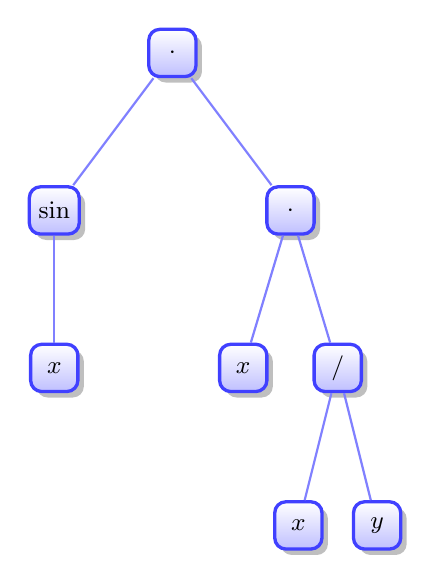
\begin{tikzpicture}
		[font=\small, edge from parent, 
		every node/.style={top color=white, bottom color=blue!25, 
			rectangle,rounded corners, minimum size=6mm, draw=blue!75,
			very thick, drop shadow, align=center},
		edge from parent/.style={draw=blue!50,thick},
		level 1/.style={sibling distance=3cm},
		level 2/.style={sibling distance=1.2cm}, 
		level 3/.style={sibling distance=1cm}, 
		level distance=2cm,
		]
		\node (A) {$\cdot$} 
		child { node (B) {$\sin$}
			%child { node {x} 
				%edge from parent node[left=.5em,draw=none] {} }
			child { node {$x$}}
		}
		child {node (C) {$\cdot$}
			%child { node {x}
				%	child { node {C1a}}
				%}
			child { node {$x$}}
			child { node {$/$}
				child { node {$x$}}
				child { node {$y$} %edge from parent node[right=.5em,draw=none] {$\frac{a}{b}$}
				}
			}
		};
		%	child { node {+} 
			%	child { node {2}}
			%	child { node {$x$}}
			%};
		
	\end{tikzpicture}
	
	\caption{Syntax tree representation for the expression $\sin{x} \cdot   ( x \cdot  x / y  )  = \frac{x^2 \sin x }{y}$}
	\label{fig:syntax-tree-example}
\end{figure}

	\section{The proposed RILS-ROLS method}\label{sec:rils}

Our method relies on the following operations: $+$, $-$, $\cdot$, $/$, $\sqrt{x}$, $x^2 $, $\sin$, $\cos$, $\log$, $\exp$, $a^x$, where $a^x$ is only consequently used -- it is never explicitly introduced in the search space. Beside these, the following set of constants enters the search space explicitly: $-1$, $0$, $1$, $2$, $\pi$, and $10$. 
Before we provide details of our method for solving SR, we will explain the two building blocks of \textsc{RILS-ROLS}: 1) iterated local search (ILS) and 2) ordinary least square (OLS). 

\subsection{Iterated local search}
ILS~\cite{lourencco2003iterated} is an efficient meta-heuristic that iteratively generates a sequence of solutions produced by the (embedded) heuristic, such as local search (LS) or randomized greedy heuristics. When the search gets \emph{stuck} in the local optimum, \emph{perturbation} is performed, which is usually a non-deterministic step. This simple idea was proposed by Baxter~\cite{baxter1981local} in the early 1980s, and has since then been re-invented by many researchers under different names. These are some of the names that were used: iterated descent search~\cite{baum1998iterated}, large-step
Markov chains~\cite{martin1991large}, chained local optimization~\cite{martin1996combining}, or in some cases, combinations of those~\cite{applegate2003chained}. The most popular version of ILS is shown in Algorithm~\ref{alg:ils}. (Note that we use this version of ILS as the backbone of our \textsc{RILS}-\textsc{ROLS} algorithm.)

\begin{algorithm}
	\begin{algorithmic}[1] 
		\State \textbf{Input}: problem instance
		\State \textbf{Output}: feasible solution 
		\State $s \gets$ \texttt{Initialize}$()$
		\State  $s \gets$ \texttt{LocalSearch}($s$)
		\While{\emph{stopping criteria are not met}}
		\State  $s' \gets$ \texttt{Perturbation}($s$)
		\State  $s' \gets$ \texttt{LocalSearch}($s'$)
		\State  $ s \gets$ \texttt{AcceptanceCriterion}($s, s'$)
		\EndWhile
		\State \Return $s$
	\end{algorithmic}
	\caption{General ILS method.}
	\label{alg:ils}
\end{algorithm}  

An initial solution may be generated randomly or by using a greedy heuristic, which is afterwards improved by local search. At each iteration, ILS applies three steps. First, the current incumbent solution $s$ is perturbed, i.e., partially randomized, yielding a new solution $s'$. Next, the solution $s'$ is potentially improved by an LS procedure. Thirdly, the newly obtained solution $s'$  possibly becomes a new incumbent -- this is decided upon the acceptance criterion. Sometimes, ILS incorporates the mechanism of a tabu list, which prevents the search from getting back into already visited solutions.  		 


\subsection{Ordinary least square method}\label{sec:ols}
The ordinary least square method (OLS) is a linear regression technique. It is based on applying the least-square method to minimize the square residual (error) sum  between actual and predicted values (given by the model). More precisely, given the   dataset $D$ of $n$ points $(\mathbf{x_i}, y_i)$ where each $\mathbf{x_i}$ is $d$-dimensional, the task is to determine linear mapping $\tilde{y} = \mathbf{k} \mathbf{x} + b$, that is coefficients (line slope) $\mathbf{k} = (k_1, \ldots, k_d)$ and $b$ (intercept), so that $ \sum_{i}^{n} (\tilde{y}_i - y_i)^2 $ is minimized. This sum is also known as the sum of squared errors (SSE). There are many methods to minimize SSE. One of the analytical approaches is calculus-oriented so it takes into account the partial derivatives of SSE w.r.t. $k_j,\; j \in \{1, ..., d\}$: 

$$  \frac{\partial}{\partial k_j} \sum_{i}^{n} (\tilde{y}_i - y_i)^2 = \frac{\partial}{\partial k_j} \sum_{i=1}^{n} ( \mathbf{k}\mathbf{x_i}+b  - y_i)^2 =  \sum_{i=1}^{n} 2x_{ij}(\mathbf{k}\mathbf{x_i} + b - y_i).$$ 

Similarly, by taking into account  partial derivation w.r.t. $b$, we have: 
$$  \frac{\partial}{\partial b} \sum_{i=1}^{n} (\tilde{y}_i - y_i)^2  = \frac{\partial}{\partial b} \sum_{i=1}^{n} ( \mathbf{k}\mathbf{x_i}+b  - y_i)^2 = \sum_{i=1}^{n} -2  (y_i - \tilde{y}_i). $$

Finally, by setting each partial derivative to zero, we get the system of $d+1$ linear equations with $d+1$ unknowns ($\mathbf{k}=(k_1, ..., k_d)$ and $b$): 
 
 \begin{align*}
	& \sum_{i=1}^{n} -2x_{i1} (y_i - \tilde{y}_i) = 0 \\
	& \vdots \\
	& \sum_{i=1}^{n} -2x_{id} (y_i - \tilde{y}_i) = 0 \\
	&\sum_{i=1}^{n} -2  (y_i - \tilde{y}_i) = 0.
\end{align*} 


%https://www.thekerneltrip.com/machine/learning/computational-complexity-learning-algorithms/
%https://math.stackexchange.com/questions/84495/computational-complexity-of-least-square-regression-operation %https://levelup.gitconnected.com/train-test-complexity-and-space-complexity-of-linear-regression-26b604dcdfa3
To solve this system, one can use Cholesky  factorization or LU decomposition for matrix inversion, and Winograd or Strassen algorithm for matrix multiplication, depending on a solver of linear equations chosen as well as the sparsity of the matrix associated with the linear system~\cite{krishnamoorthy2013matrix}. For example, by using Cholesky decomposition, solving the system requires matrix inversions and matrix multiplications. In that case the computation cost of $O(d^3)$ is required to find an inverse of the matrix associated to the linear system, which is the most consuming part of the algorithm. Thus, the OLS that use close-form matrix techniques perform in $O(d^3)$ time complexity.  %, where $d$ stands for the number of input features. 
It is worth mentioning that when the number of input features becomes large, these closed-form matrix techniques are usually replaced by iterative ones, such as gradient descent (GD)~\cite{andrychowicz2016learning}. When using GD the complexity becomes $O(n^2d )$.
% The learning rate in GD has to be carefully chosen, as it dictates how quick the algorithm is and how fast it converges. 


\subsection{\textsc{RILS}-\textsc{ROLS}  method}
We will now explain the proposed \textsc{RILS}-\textsc{ROLS} method in detail. The overall method scheme is given in Algorithm~\ref{alg:rilsrols}.   

\begin{algorithm}
	\footnotesize

	\begin{algorithmic}[1] 
		\Statex	  \textbf{Input}: input training dataset $D_{tr}$  
		\Statex \textbf{Control parameters}: size penalty $penalty_{size}$, error tolerance $tolerance_{error}$  
		\Statex \textbf{Output}: best symbolic formula solution $bs$
		\Procedure{\textsc{RILS}-\textsc{ROLS} }{$D_{tr}$}
		\State $n_{tr} \gets |D_{tr}|$
		\State $sample_{size} \gets $ \texttt{InitialSampleSize}($n_{tr}$)
		\State $D_{tr}' \gets$ \texttt{Sample}($D_{tr}, sample_{size}$)
		\State $s \gets NodeConstant(0)$ 
		\State $s_{fit} \gets$ \texttt{Fitness}($s, D_{tr}'$)
		\State $bs, bs_{fit} \gets s, s_{fit}$ \label{line:solSet}
		\State $start_{tried}, perturbations_{tried} \gets \emptyset, \emptyset$
		\While{\emph{stopping criteria is not met}}
		\State $start_{tried} \gets start_{tried} \cup \{s\}$
		\State $s_{perturbations} \gets $ \texttt{All1Perturbations}($s$) \label{line:sPert}
		\State $s_{perturbations} \gets $ \texttt{FitOLS}($s_{perturbations}$, $D_{tr}'$)
		\State $s_{perturbations} \gets $ \texttt{OrderByR2}($s_{perturbations}$) \label{line:orderR2}
		\State $improved \gets false $
		\For{$p \in s_{perturbations}$}
		\If{$p \in perturbations_{tried}$}
		\State \textbf{continue}
		\EndIf
		\State $p \gets $ \texttt{Simplify}($p$) \label{line:simp}
		\State $p \gets $ \texttt{LocalSearch}($p$, $D_{tr}'$) \label{line:ls}
		\State $p_{fit} \gets$ \texttt{Fitness}($p$, $D_{tr}'$)
		\If{$p_{fit} < bs_{fit}$} \label{line:avoid1}
		\State $bs, bs_{fit}, improved \gets p, p_{fit}, true$ // new best solution
		\State \textbf{break}
		\EndIf \label{line:avoid2}
		\State $perturbations_{tried} \gets perturbations_{tried} \cup \{p\}$
		\EndFor
		\If{improved}
		\State $s \gets bs$ \label{line:improved}
		\Else
		\State $start_{candidates} \gets $ \texttt{All1Perturbations}($bs$)
		\If{$start_{candidates} \setminus start_{tried} = \emptyset$} // all 1-perturbations around $bs$ tried
		\State $s' \gets $ \texttt{RandomPick}($start_{candidates}$)  \label{line:pert21}
		\State $start_{candidates} \gets $ \texttt{All1Perturbations}($s'$) \label{line:pert22} // 2-permutations of \textit{bs}
		\EndIf
		\State $s \gets $ \texttt{RandomPick}($start_{candidates} \setminus start_{tried}$) \label{line:randPick}
		\If{not improved for too many iterations}
		\State $sample_{size} \gets$ \texttt{IncreaseSampleSize}($sample_{size}, n_{tr}$) \label{line:sampleAdj1}
		\State $D_{tr}' \gets$ \texttt{Sample}($D_{tr}, sample_{size}$)\label{line:sampleAdj2}
		\EndIf
		\EndIf
		\If{$R^2$ almost 1 and RMSE almost 0 w.r.t. $tolerance_{error}$}
		\State \textbf{break} // early exit
		\EndIf
		\EndWhile
		\State $bs \gets $ \texttt{Simplify}($bs$)
		\State $bs \gets $ \texttt{RoundModelCoefficients}($bs$)
		\State \Return $bs$
		\EndProcedure
	\end{algorithmic}
	\caption{\textsc{RILS}-\textsc{ROLS}  method.}
	\label{alg:rilsrols}
\end{algorithm}  

The \textsc{RILS}-\textsc{ROLS} algorithm receives the training dataset $D_{tr}$ as input. In addition, it has two control parameters: $penalty_{size}$ and $tolerance_{error}$. The first one quantifies the importance of solution expression complexity in the overall solution quality measure (more on this in Section~\ref{sec:fitness}). The second parameter is related to the expected noise level in data whereby higher noise means that tolerance to errors should be higher.
$D_{tr}$ can have a very large number of records, so the first step of \textsc{RILS}-\textsc{ROLS}  is to choose a random sample $D_{tr}' \subseteq D_{tr}$ of size $sample_{size}$. Initially, sample size is chosen as $\max(0.01 \cdot n_{tr}, 100)$. The size of the sample is later dynamically adjusted through the algorithm's iterations -- when there are no solution improvements for a number of iterations, sample size is doubled (lines~\ref{line:sampleAdj1}-\ref{line:sampleAdj2} of Algorithm~\ref{alg:rilsrols}).

As previously stated, solution is usually represented by means of a tree. We use a simple solution initialization where the tree root node is set to zero constant. We interchangeably use two solution variables: ($i$) $s$ denotes the starting (or working) solution and ($ii$) $bs$ stands for the best solution so far, also known as the incumbent solution. Solution quality is measured by evaluating the fitness function (more about it in the subsequent Section~\ref{sec:fitness}). Before entering the main loop, the best solution \emph{bs} is set to the initial solution (line~\ref{line:solSet}). 


The main loop iterates as long as none of the termination criteria are met: ($i$) the maximal running time has been reached; ($ii$) the maximal number of fitness calculations has been made; ($iii$) the best solution is sufficiently good 
w.r.t. its $R^2$ and $RMSE$ scores. More precisely, if $R^2$ is sufficiently close to 1 and, at the same time $RMSE$ is sufficiently close to 0, the algorithm stops prematurely, which significantly reduces the running times for the majority of tested instances.
The sufficiency is controlled with parameter $tolerance_{error}$, whereby a smaller value means that $R^2$ and $RMSE$ should be closer to 1 and 0, respectively. 


One of the first steps in the main loop is to generate perturbations near the starting solution $s$ (line~\ref{line:sPert}). 
As the name of this procedure (\texttt{All1Perturbations}) suggests, the perturbation step is local, meaning that the closeness of the starting solution $s$ and any of perturbations is 1 (we sometimes call it 1-perturbation). The precise way of generating perturbation is described separately in Section~\ref{sec:pertGen}. 


Candidate perturbations are improved by performing OLS coefficient fitting (procedure \texttt{FitOLS}). This means that the coefficients in any of the linear combinations of the current solution are being set by applying the ordinary least square method already described in Section~\ref{sec:ols}. 
After this step, perturbations are usually better suited to the given sample data $D_{tr}'$. 
Further, these perturbations are sorted w.r.t. $R^2$ metric in the descending order (line~\ref{line:orderR2}). 

Now the algorithm enters the internal loop -- it iterates over the ordered perturbations and aims to find the one which improves the best solution $bs$. But before comparing candidate perturbation solution $p$ with $bs$, $p$ is first simplified (line~\ref{line:simp}), after which local search is performed (line~\ref{line:ls}).
Solution simplification is done in a symbolic fashion by popular  Python package \texttt{SymPy}~\cite{sympy}.
The local search tries to find local optima expressions close to the given $p$, explained in detail in Section~\ref{sec:ls}.  
Finally, the fitness function value of $p$ is compared to the fitness function value of $bs$. If fitness of $p$ is better, $bs$ is updated correspondingly and the internal loop, which goes across ordered perturbations, is immediately terminated (it works in a  \emph{first-improvement} strategy). Otherwise, the next perturbation is probed. 
Note that the probed perturbations are stored in a set denoted by $perturbations_{tried}$. The goal is to avoid checking the same perturbation multiple times (lines \ref{line:avoid1}-\ref{line:avoid2}), i.e., $perturbations_{tried}$ serves as a kind of tabu list, which is known from the Tablu search meta-heuristic (see~\cite{glover1998tabu}).    


If some of $s_{perturbations}$ around the starting solution $s$ yielded an improvement, $bs$ becomes the starting solution $s$ in the next iteration of the main loop (line~\ref{line:improved}). 
Otherwise, it makes no sense to set the starting solution to $bs$ as the search becomes  \emph{trapped} in a local optimum. Randomness is introduced in order to avoid this undesirable situation. First, a set of local perturbations around $bs$ is generated ($start_{candidates}$) in the same manner as before (procedure \texttt{All1Perturbations}). If at least one of these was not previously used as a starting solution ($start_{tried}$), a single perturbation from the $start_{candidates} \setminus start_{tried}$ is randomly picked (line~\ref{line:randPick}). There is a minor chance that $start_{candidates} \setminus start_{tried} = \emptyset$. When that happens, the set of starting solution candidates is equal to perturbations of some randomly selected perturbation of $bs$ (lines \ref{line:pert21}-\ref{line:pert22}) -- which effectively means that the perturbations with distance 2 from $bs$ are used. There is a very small chance that these 2-perturbations will have an empty set difference with $start_{tried}$ set of starting solutions. Therefore, 3-perturbations are not considered in our algorithm. 

Before returning the symbolic model, \textsc{RILS}-\textsc{ROLS}  performs the final symbolic simplification and rounding of model coefficients. The latter is sensitive to control parameter $tolerance_{error}$ -- a smaller value means that information loss during rounding is smaller, i.e., a higher number of significant digits is preserved. Note that confidence in the symbolic model is reduced when expected noise in data is higher; the rule of thumb is: for higher expected noise, $tolerance_{error}$ should be higher. 


\subsubsection{Fitness function}\label{sec:fitness}


The objective of symbolic regression is to determine the expression that fits available data. It is also allowed to obtain an equivalent expression, since there are multiple ways to express a symbolic equation. Although logically sound and intuitive, this objective is not quantifiable during the solution search/training phase, because the goal expression is not known at that point but only target values for some of the input data. Therefore there are various numerical metrics in the literature that guide the symbolic regression search process. The most popular ones are the coefficient of determination, also known as $R^2$, and the mean squared error (MSE) or root mean squared error (RMSE). The important aspect of solution quality is solution expression complexity, which may correspond to the model size of its tree representation. This follows the Occam's razor principle~\cite{costa2020fast} that a simpler solution  is more likely to be the correct one. 
The search process of \textsc{RILS}-\textsc{ROLS}  is guided by the non-linear combination of $R^2$, RMSE, and solution expression size (complexity) presented in Equation~(\ref{eq:fitness}). 

\begin{equation}
	\label{eq:fitness}
	fit(s) = (2-R^2(s)) \cdot (1+RMSE(s)) \cdot (1+penalty_{size} \cdot size(s))
\end{equation}

Since the presented fitness function needs to be minimized, the following conclusions may be drawn:
\begin{itemize}
	\item higher $R^2$ is preferred, ideally when $R^2(s)=1$, the effect of term $2-R^2(s)$ is neutralized; %since 1 is neutral for multiplication;
	\item lower RMSE is preferred, ideally when $RMSE(s)=0$, the whole term $(1+RMSE(s))$ becomes 1;
	\item since $penalty_{size} > 0$, larger expressions tend to have higher fitness (which follows the Occam's razor principle); therefore, simpler solutions are favorable. 
\end{itemize}

The size of expression is calculated by counting all nodes in the expression tree -- this includes leaves (variables and constants) and internal nodes (operations). 

\subsubsection{Expression caching}

In order to speed up fitness evaluation, we employ \emph{expression caching}. This means that values attached to expression trees or subtrees are stored in key-value structure, such that the key is tree (subtree) textual representation, while the value is the $|D_{tr}'|$-size  vector of corresponding expression values on the sample training dataset $D_{tr}'$. Of course, once the $D_{tr}'$ changes, which does not happen very frequently, the whole cache is cleared.
Caching is performed in a partial way -- when determining the value of a given expression $T$, it is not required to find the exact \emph{hit} inside the cache. So, if a subexpression (subtree) of $T$ is present in the cache, its value will be reused and further combined to calculate the whole fitness function value. 

For example, let  $T = y^2 \cdot (x+y)/z - \sin(x+y)$ be an expression, and $D_{tr}'=\{([1, 2, 5], 7), ([3, 4, 3], 5), ([4, 5, 3], 6), ([6, 7, 4], 3), ([3, 3, 6], 2)\}$ be a sample training dataset (here, input feature vector is labeled by $[x, y, z]$); let expression cache consist of the following key-value entries $cache=\{(x+y, [3, 7, 9, 13, 6]), (y^2, [4, 16, 25, 49, 9])\}$.  
Expression $T$ does not need to be fully evaluated since some of its parts are inside the cache: $y^2$ and $x+y$. Note that single variables do not need to enter the cache, since they are already available as columns of  $D_{tr}'$.
Each newly evaluated (sub)expression (except for the constant or variable alone) enters the cache. In this example, the new entries will correspond to keys $(x+y)/z$, $y^2 \cdot (x+y)/z$, $\sin(x+y)$ and $y^2 \cdot (x+y)/z - \sin(x+y)$.  
The maximal number of cache entries is set to 5000. Once this number is reached, the cache is cleared. 

\subsubsection{Perturbations}\label{sec:pertGen}

Perturbations allow the algorithm to escape from local optima. As previously described, perturbations are performed on two occasions: ($i$) during the exhaustive examination of neighboring solutions around the starting solution, ($ii$) during selection of the next starting solution, a non-exhaustive case.  
In both cases, the same Algorithm~\ref{alg:pert} is used. 

\begin{algorithm}
    
	\begin{algorithmic}[1] 
		\Statex   \textbf{Input}: solution $s$ 
		\Statex \textbf{Output}: local perturbations (1-perturbations) of solution $s$ -- $s_{perturbations}$
		\Procedure{All1Perturbations}{$s$}
		\State $s_{perturbations} \gets \emptyset$ \label{line:pertInit}
		\State $s \gets$ \texttt{NormalizeConstants}($s$)
		\State $s \gets$ \texttt{Simplify}($s$)
		\State $s_{subtrees} \gets$ \texttt{SubTrees}($s$)
		\For{$n \in s_{subtrees}$} \label{line:forSSStart}
		\State $n_{perturbations} \gets$ \texttt{All1PerturbationsAroundNode}($s$, $n$)
		\State $s_{perturbations} \gets s_{perturbations} \cup n_{perturbations}$	
		\EndFor \label{line:forSSEnd}
		\State \Return $s_{perturbations}$
		\EndProcedure
	\end{algorithmic}
	\caption{Generation of all 1-perturbations of a given solution.}
	\label{alg:pert}
\end{algorithm}  

Initially, the set of perturbations $s_{perturbations}$ is empty (line~\ref{line:pertInit} of Algorithm~\ref{alg:pert}).


This is followed by constant normalization during which coefficients that enter multiplication, division, addition or subtraction are set to 1, while those entering the power function are rounded to integer, with the exception of square root, which is kept intact. For example, for expression $3.3\cdot(x+45.1\cdot y^{3.2})\cdot 81\cdot x/\sqrt{y}$ the normalized version is $1\cdot (x+1\cdot y^3)\cdot 1\cdot x/\sqrt{y}$. The reason for performing normalization is reducing the search space of possible perturbations. This reduction is reasonable, since normalization preserves the essential functional form. Note that coefficients get tuned later: the linear coefficient during the OLS phase, and the remaining ones during local search, see Section~\ref{sec:ls}. 


After performing the normalization process, the expression is simplified -- getting the compact expression is more likely after normalization than before it. The previous expression will take the form $(x+y^3)\cdot x/\sqrt{y}$. In this particular case, the simplification will usually only remove unnecessary coefficients, but in general it can also perform some non-trivial symbolic simplification. 


Perturbations are generated by making simple changes on the per-node level of $s$ expression tree.
Depending on the structure of the expression tree (note that the expression does not need to have unique tree representation), the set of subtrees of the previous expression $(x+y^3)\cdot x/\sqrt{y}$ might be $\{(x+y^3)\cdot x/\sqrt{y}, (x+y^3), x/\sqrt{y}, x, y^3, \sqrt{y}, y\}$. %This set of subtrees is obtained if left subtree of the whole expression is $(x+y^3)$ while the right one is $x/\sqrt{y}$.  
Further, the set of perturbations is generated around each subtree $n$ (lines \ref{line:forSSStart}-\ref{line:forSSEnd} in Algorithm~\ref{alg:pert}).   


Algorithm~\ref{alg:pertNode} shows how perturbations are generated around the given subtree.

\begin{algorithm}	
	 
	\begin{algorithmic}[1]
		\Statex  \textbf{Input}: solution $s$, node $n$ 
		\Statex  \textbf{Output}: 1-perturbations of solution $s$ around node $n$
		\Procedure{All1PerturbationsAroundNode}{$s$, $n$}
		\State $n_{perturbations} \gets \emptyset$
		\If{$n = s$} \label{alg:alg4-case-1}
		\State $n_{perturbations} \gets n_{perturbations} \cup$ \texttt{NodeChanges}($n$)
		\EndIf
		\If{$n.arity \geq 1$}\label{alg:alg4-case-2}
		\State $n_{changes} \gets$ \texttt{NodeChanges}($n.left$)
		\For{$nc \in n_{changes}$}
		\State $new \gets$ \texttt{Replace}($s$, $n.left$, $nc$)
		\State $n_{perturbations} \gets n_{perturbations} \cup \{new\}$
		\EndFor
		\EndIf
		\If{$n.arity = 2$}\label{alg:alg4-case-3}
		\State $n_{changes} \gets$ \texttt{NodeChanges}($n.right$)
		\For{$nc \in n_{changes}$}
		\State $new \gets$ \texttt{Replace}($s$, $n.right$, $nc$)
		\State $n_{perturbations} \gets n_{perturbations} \cup \{new\}$
		\EndFor
		\EndIf
		\State \Return $n_{perturbations}$
		\EndProcedure
	\end{algorithmic}
	\caption{Generation of 1-perturbations of a given solution around given node.}
	\label{alg:pertNode}
\end{algorithm}

It can be seen that there are three possibly overlapping cases when performing perturbations on the per-node level. 

\emph{Case 1}. 
The observed node $n$ is the whole tree $s$ (see line~\ref{alg:alg4-case-1} in Algorithm~\ref{alg:pertNode}). Based on  the previous exemplary expression tree, this means that the multiplication node that connects $(x+y^3)$ and $x/\sqrt{y}$ is to be changed. For example, multiplication can be replaced by addition, which forms a 1-perturbation expression (tree) $(x+y^3)+ x/\sqrt{y}$. 


\emph{Case 2}. 
Node $n$ has the arity of at least 1 (see line~\ref{alg:alg4-case-2} in Algorithm~\ref{alg:pertNode}). This means that the left subtree exists, so the left subtree node is to be changed. 
For example, if $n=x+y^3$, the overall perturbation might be $(x/y^3)+x/\sqrt{y}$ (addition is replaced by division). 
Another example would be the case of unary operation, e.g., when $n=\sqrt{y}$. In that case, some possible perturbations could be $(x+y^3)\cdot x/\sqrt{\ln{y}}$ (application of logarithm to the left subtree $y$) or $(x+y^3)\cdot x/\sqrt{x}$ (changing variable $y$ to $x$), etc.

\emph{Case 3}. 
Node $n$ is a binary operation, meaning that the right subtree must exist (Line ~\ref{alg:alg4-case-3} in Algorithm~\ref{alg:pertNode}). 
The analogous idea is applied as in \emph{Case 2}. 

The algorithm allows for the following set of carefully chosen per-node changes (method named \texttt{NodeChanges} in Algorithm~\ref{alg:pertNode}): 

\begin{enumerate}
	\item Any node to any of its subtrees (excluding itself). For example, if $(x+y^3)$ is changed to $x$, the perturbation is $(x+y^3)\cdot x/\sqrt{y} \rightarrow x\cdot x/\sqrt{y}$. 
	\item Constant to variable. For example,  $(1+y^3)\cdot x/\sqrt{y} \rightarrow (x+y^3)\cdot x/\sqrt{y}$.
	\item Variable to the unary operation applied to that variable. For example,  $(x+y^3)\cdot x/\sqrt{y} \rightarrow (x+y^3)\cdot \ln{x}/\sqrt{y}$.
	\item Unary operation to another unary operation. For example,  $(x+y^3)\cdot x/\sqrt{y} \rightarrow (x+y^3)\cdot x/\sin{y}$.
	\item Binary operation to another binary operation. For example,  $(x+y^3)\cdot x/\sqrt{y} \rightarrow (x+y^3)\cdot (x + \sqrt{y})$. 
	\item Variable or constant enter the binary operation with an arbitrary variable. For example,  $(x+y^3)\cdot x/\sqrt{y} \rightarrow (x+x/y^3)\cdot x/\sqrt{y}$. 
\end{enumerate}

The method named \texttt{Replace}$(s, n, nc)$ inside Algorithm~\ref{alg:pertNode} is simply used to replace the node $n$ with node $nc$ inside the given expression tree $s$.   

\subsubsection{Local search}\label{sec:ls}

Perturbations are further improved by means of the local search procedure (Algorithm~\ref{alg:ls}). 

\begin{algorithm}
 
	\begin{algorithmic}[1] 
		\Statex \textbf{Input}: perturbation $p$, sample training dataset $D_{tr}'$   
		\Statex \textbf{Output}: local optimum $bp$ in the vicinity of perturbation $p$
		\Procedure{LocalSearch}{$p$, $D_{tr}'$}
		\State $bp, bp_{fit} \gets p,\ $\texttt{Fitness}$(p,D_{tr}')$ 
		\State $improved \gets true$
		\While{$improved$}
		\State $improved \gets false$
		\State $bp_{candidates} \gets \emptyset$
		\State $bp_{subtrees} \gets $\texttt{SubTrees}($bp$)
		\For{$n \in bp_{subtrees}$}
		\State $n_{candidates} \gets $ \texttt{All1PerturbationsAroundNodeExtended}($bp$, $n$)
		\For{$new \in n_{candidates}$}
		\State $new \gets$ \texttt{FitOLS}($new$, $D_{tr}'$)
		\State $new_{fit} \gets$ \texttt{Fitness}($new$, $D_{tr}'$)
		\If{$new_{fit} < bp_{fit}$}
		\State $bp, bp_{fit} \gets new, new_{fit}$
		\State $improved \gets true$
		\EndIf
		\EndFor
		\EndFor
		\EndWhile
		\State \Return $bp$
		\EndProcedure
	\end{algorithmic}
	\caption{Local search procedure.}
	\label{alg:ls}
\end{algorithm}  

For a given perturbation $p$, local search systematically explores the extended set of 1-perturbations around $p$. It relies on the \emph{best-improvement} strategy, meaning that all 1-perturbations (for all subtrees) are considered. Before checking if the candidate solution ($new$) is better than the actual best $bp$, the OLS coefficient fitting (\texttt{FitOLS}) takes place.  


The set of used 1-perturbations is expanded in comparison to those used previously. Namely, in addition to those six possible types of node changes, the following four are added:

\begin{enumerate}
	\setcounter{enumi}{6}
	\item Any node to any constant or variable. For example, $(x+y^3)\cdot x/\sqrt{y} \rightarrow y \cdot x / \sqrt{y}$ or  $(x+y^3)\cdot x/\sqrt{y} \rightarrow (x+\pi) \cdot x / \sqrt{y}$.
	\item Any node to the unary operation applied to it. For example, $(x+y^3)\cdot x/\sqrt{y} \rightarrow (x+y^3)\cdot x/\ln{\sqrt{y}}$.
	\item Any node to the binary operation applied to that node and a variable or constant. For example, $(x+y^3)\cdot x/\sqrt{y} \rightarrow (x+y^3)\cdot x/\sqrt{y} - x$.
	\item Constant to its multiple, whereby possible multipliers are $\{$0.01, 0.1, 0.2, 0.5, 0.8, 0.9, 1.1, 1.2, 2, 5, 10, 20, 50, 100$\}$. For example, $(1+y^3)\cdot x/\sqrt{y} \rightarrow (1.2+y^3)\cdot x/\sqrt{y}$.
\end{enumerate}

Change under point 10 is very important as it performs general coefficient tuning, unlike OLS, which considers only coefficients in linear combinations.  

\section{Experimental evaluation}\label{sec:experiments}

Our \textsc{RILS}--\textsc{ROLS} algorithm is implemented in Python 3.9.0. All experiments concerning our method are conducted in the single-core mode, on a PC with Intel i9-9900KF CPU @3.6GHz, 64GB RAM, under Windows 10 Pro OS. The RAM consumption was very small (up to a few hundred megabytes). Beside the memory space needed to load the input dataset, the only considerable amount is reserved for expression cache. 


The following 14 algorithms are compared to our approach: \textsc{AI-Feynman}, \textsc{GOMEA}, \textsc{Afp-Fe}, \textsc{Itea}, \textsc{Afp}, \textsc{Dsr}, \textsc{Operon}, the \textsc{gplearn} from python package \textsc{gplearn}~\cite{stephens2016genetic}, \textsc{Sbp-Gp}, \textsc{Eplex}, \textsc{Bsr}, \textsc{Feat}, \textsc{Ffx}, \textsc{Mrgp}. 

For the 14 competitors, the results are exported from \texttt{SRBench} \url{https://cavalab.org/srbench/results/}, reported in~\cite{la2021contemporary}. 
The maximum computation time allowed for each run of \textsc{RILS}-\textsc{ROLS} is set to 1 hour, while the maximal number of fitness function evaluations is set to 1 million. All other algorithms from \texttt{SRBench} used the time limit that was equal to or below 8 hours runtime and the same fitness evaluation limit of 1 million (see~\cite{la2021contemporary}). We did not use the full time limit of 8 hours because we empirically concluded that there were almost no improvements after 1 hour \textsc{RILS}-\textsc{ROLS} runtime.

All non-deterministic algorithms (including \textsc{RILS}-\textsc{ROLS}) were run ten times per each problem instance, where each run used a different setting of a random number generator seed. 

The training/test data splits were randomly performed in ratio 75\%:25\%, the same as in \texttt{SRBench}. Moreover, the splits are structurally the same as in \texttt{SRBench}, because we used the same set of random number generator seeds and the same Python splitting method (\texttt{train\_test\_split} from Scikit-Learn library~\cite{scikit-learn}). 

\subsection{Datasets and \texttt{SRBench}}

\texttt{SRBench} (\url{https://cavalab.org/srbench/}) is an open-source benchmarking project which merges a large set of diverse benchmark datasets, contemporary SR methods, as well as ML methods around shared model evaluation and an environment for analysis (see~\cite{la2021contemporary}). \texttt{SRBench} considers two types of symbolic regression problems: 1) ground-truth problems, for which the exact model is known, and 2) black-box problems, for which the exact model is not known. In our work, we consider only the former one, since \textsc{RILS-ROLS} was not designed to solve black-box problems. There are two groups of instances in the \texttt{SRBench} ground-truth problem set:
\begin{itemize}
	\item \textsc{Feynman} instances are inspired by physics and formulas/models that describe various natural laws.  
	There are 116 instances, where each one consists of $10^5$  samples (see \cite{udrescu2020ai} for more details). Some exact models (equations) of \textsc{Feynman} instances are listed in Table~\ref{tab:Feynamn-Eq}.  
	
	\begin{table}[!ht]
		\caption{Some \textsc{Feynman} instances.}
		\label{tab:Feynamn-Eq}
		\centering
		\begin{tabular}{l}   \hline
			$x = \sqrt{x_1^2 + x_2^2 - 2 x_1 x_2 \cos(\theta_1 - \theta_2)}$ \\
			$ \theta_1 = \arcsin(n \sin \theta_2)$ \\
			$E =  \frac{m c^2 }{1 - \frac{v^2}{c^2}}$ \\
			$\omega = \frac{1 + \frac{v}{c}}{ \sqrt{1 - \frac{v^2}{c^2}}} \omega_0$ \\ \hline
			
		\end{tabular}
	\end{table}
	
	\item \textsc{Strogatz} instances are introduced in \cite{la2016inference}. 
	Each instance represents a 2-state system of first-order, ordinary differential equations. 
	The aim of each problem is to predict the rate of change of the subsequent state. These equations describe the natural processes modeled by non-linear dynamics exhibiting chaos.  The equations for some of the datasets that belong \textsc{Strogatz} are shown in Table~\ref{table:strogatz-ODEs}. There are 14 \textsc{Strogatz} instances in total. 
	
	%table, an instance -- example
	
	\begin{table}
		\caption{Some \textsc{Strogatz} ODE instances.}
		\label{table:strogatz-ODEs}
		\centering
		\begin{tabular}{ll} \\ \hline
			Bacterial representation &   $x' = 20 - x - \frac{x \cdot y}{1 + 0.5 x^2 }$ \\ 
			&   $y' = 10 - \frac{x \cdot y}{1 + 0.5 x^2  }$ \\ \hline
			Shear Flow               &  $\theta' = \cot(\phi)\cos(\theta)$ \\
			&  $ \phi'  = ( \cos^2(\phi) + 0.1 \cdot \sin^2 (\phi)) \sin(\theta) $ \\ \hline
		\end{tabular}
	\end{table}
	
\end{itemize}

The above-mentioned benchmark sets may be biased since the models which describe physical laws usually impose various symmetries, periodicity, or internal separability on some variables, etc. In order to test \textsc{RILS-ROLS} robustness and scalability in unbiased setting, we generated a set of random SR problem instances called \textsc{Random}. These instances vary in size (total number of expression nodes) and number of variables. In total, there are 235 random instances, or 5 randomly generated instances for each of the following 47 (size, number of variables) combinations $\{(3, 1), \{4, 5\} \times \{1, 2\}, \{6\} \times \{1, 2, 3\}, \{7, 8, 9, 10, 11, 12\} \times \{1, 2, 3, 4\}, \{13, 14, 15\} \times \{1, 2, 3, 4, 5\}\}$. Each of the \textsc{Random} instances has 10,000 randomly generated samples. 

Some random instances are shown in Table~\ref{table:random}, while all instances can be found in %\textsc{RILS-ROLS} GitHub 
 the following repository: \url{https://github.com/kartelj/rils-rols}.  

\begin{table}
	\caption{Some \textsc{Random} instances.}
	\label{table:random}
	\centering
	\begin{tabular}{ll} \\ \hline
		random\_04\_02\_0010000\_00 &	$\ln{(x_0 + x_1)}$\\
		random\_07\_02\_0010000\_00 &	$(x_0 + 10)\cdot (x_1 + 1)$\\
		random\_08\_02\_0010000\_00 &	$(x_0 + \ln{x_0})*(x_1 + 10)$\\
		random\_10\_03\_0010000\_02 &	$\ln{(\sqrt{x_0} \cdot x_1/\cos{x_2})}$\\
		random\_12\_04\_0010000\_04 &	$\sqrt{x_3 \cdot \exp{x_1} + \cos{(x_2 \cdot \sin{x_0})}}$\\
		random\_15\_03\_0010000\_04	&   $x_0 \cdot x_1/2 + (\cos{(x_2)} - \pi^2)^2$\\
		\hline
	\end{tabular}
\end{table}

\subsection{Parameter tuning}

The \textsc{RILS}-\textsc{ROLS} algorithm employs two control parameters: $penalty_{size}$ and $tolerance_{error}$. The first parameter is empirically tuned to 0.001 for considered benchmarks -- this is also used as a default value in the corresponding Python package (package is described in the Appendix). The second parameter is positively correlated with the expected level of noise in input data, i.e., for higher noise $tolerance_{error}$ should take higher values and vice-versa. More precisely, in case there is no noise, we used the default setting $tolerance_{error}=10^{-16}$, while in noisy scenarios we set $tolerance_{error}$ to the corresponding noise level (0.001 or 0.01). 
For setting $penalty_{size}$ and $tolerance_{error}$ on new datasets, one can either keep the default settings or use a wrapper tuning algorithm around the \textsc{RILS-ROLS} regressor, e.g., grid-search w.r.t. training or validation accuracy. 

\subsection{Comparison to other methods}
% ACA: ima 14 uporednih algoritama, ne 13
In this section we evaluate our \textsc{RILS-ROLS} algorithm and compare it to 14 other competitors from the literature. The numerical results are reported in Tables~\ref{tab:comp_noise0}-\ref{tab:comp_noise001}. The results for \textsc{Feynman} and \textsc{Storgatz} benchmark are given w.r.t.\  the following levels of noise: 0.0 (no-noisy data), 0.001 (low-level noise), and 0.01 (high-level noise). More precisely, the white Gaussian noise is added to the target variable the same way as in~\cite{la2021contemporary}:
$$ y_{noise} = y + \epsilon, \epsilon \sim \mathcal{N}\left(0, \alpha \sqrt{\frac{1}{n} \sum _{i=1}^n{y_i^2}}\right),$$
where $n$ relates to the number of items in input data.

Each table consists of two blocks, where the first one provides the exact model accuracy, while the second one is related to the less relevant statistical accuracy based on the $R^2$ metric. The exact model accuracy shows how often the method reaches the true formula (ground-truth). Regarding statistical accuracy, the solution is considered accurate if it produced an $R^2$ score larger than 0.999.  Note that for each instance there were 10 runs, so in total there were at most 1160 successful runs for \textsc{Feynman} and 140 for \textsc{Strogatz}.  

The following conclusions may also be drawn from the numerical results: 

\begin{itemize}
	\item Concerning the exact percentages in case when no noise is utilized in input data, the best performing algorithm is our \textsc{RILS-ROLS}. It found the exact solution in 57.84\% of runs for \textsc{Feynman} instances. It is even more impressive in solving \textsc{Strogatz} instances, as it was successful in 83.57\% runs. The second best performing  approach is \textsc{AI-Feynman}, successful in 55.78\% runs for the \textsc{Feynman} set, and 27.14\% runs for the problem instances from the benchmark set \textsc{Strogatz}. All other approaches perform significantly worse, and none of them are able to deliver the exact solution in more than 30\% runs over the instances of any of the two considered ground-truth benchmark sets. The overall results are in favor of \textsc{RILS-ROLS} with 60.62\%, while the second best is \textsc{AI-Feynman} with 52.65\%. 
	\item  Concerning the exact results in the presence of small noise (0.001), our \textsc{RILS-ROLS} still performs well, finding the exact model in 42.08\% of runs considering all problem instances. The second best approach is again \textsc{AI-Feynman}, successful in 31.89\% runs. As in the no-noise scenario, there is a significant difference in \textsc{AI-Feynman} performances among two sets of instances -- it performs much better on \textsc{Feynman} instances than on \textsc{Strogatz}. It is also worth mentioning that \textsc{AFP-FE} shows to be robust w.r.t. noise so its performances only slightly deteriorate in comparison to the no-noise scenario. This puts it on the third place with the overall accuracy of 21.23\%. The accuracy of other approaches is below 20\%.  
	\item  Concerning the scenario with high noise (level of 0.01), our \textsc{RILS-ROLS} still performs quite well -- it finds and exact model in 34.77\% runs. The second best is \textsc{AFP-FE}, reaching 20\% correct solutions. \textsc{AI-Feynman} performances degrade significantly under this level of noise, so it is the 6-th overall ranking, reaching the accuracy of only 12.61\%. 
	
	\item Another interesting method is \textsc{DSR}. It shows the perfect robustness to noise and agnosticism to the benchmark dataset -- it has almost 19\% exact model accuracy in all 6 combinations of the benchmark dataset (\textsc{Feynman} or \textsc{Strogatz}) and noise level (0, 0.001 or 0.01).     
	
	\item When comparing the performances of algorithms in terms of $R^2 > 0.999$ accuracy, in a no-noise scenario, our \textsc{RILS}-\textsc{ROLS} is successful with the success rate of 83.38\% (ranked third). Better methods in terms of this accuracy are \textsc{MRGP}, and \textsc{Operon}, with 92.69\%, and 86.92\%, respectively. On the other hand, the exact model percentages of these two approaches are rather low: 0\% and 16\%, respectively. These two algorithms are therefore more appropriate for the so-called black-box regression, i.e., scenarios when the underlying (ground-truth) model is unknown. 
	
	\item  In the presence of the noise level of 0.001, our \textsc{RILS-ROLS} method has 78.62\% success rate (ranked third, again).  As before, \textsc{MRGP} and \textsc{Operon} are best two here. 
	
	\item   When the noise level is 0.01, the situation is almost the same. \textsc{MRGP} and \textsc{Operon} are the best and second best with 88.46\% and 86.54\% accuracy, respectively. \textsc{GP-GOMEA} now reaches the third place with 73.46\%, while the proposed \textsc{RILS-ROLS} is 5-th with 62.92\% $R^2$ accuracy.
	
	\item We can conclude that \textsc{RILS}-\textsc{ROLS} achieves state-of-the-art performances regarding exact model accuracy. It also shows high robustness to noise. Regarding statistical accuracy, which is not so relevant for ground-truth problems, \textsc{RILS}-\textsc{ROLS} also performs quite well. 
	
\end{itemize}

\begin{table}[!h]
	\caption{Comparison without noise}\label{tab:comp_noise0}
	\centering
	\begin{tabular}{l|rrr|rrr} \hline
		& \multicolumn{3}{c|}{Exact model percentage} & \multicolumn{3}{c}{$R^2 > 0.999$ percentage}\\ \hline
		Method &  \textsc{Feynman} & \textsc{Strogatz}& Total &  \textsc{Feynman} & \textsc{Strogatz} & Total \\ \hline
		\textsc{RILS-ROLS}&\bf{57.84}&\bf{83.57}&\bf{60.62}&82.59&90&83.38\\
		\textsc{AI-Feynman}&55.78&27.14&52.65&78.51&35.71&73.83\\
		\textsc{GP-GOMEA}&26.83&29.46&27.12&71.55&71.43&71.54\\
		\textsc{AFP-FE}&26.98&20&26.23&59.05&28.57&55.77\\
		\textsc{ITEA}&22.41&7.14&20.77&27.59&21.43&26.92\\
		\textsc{AFP}&21.12&15.18&20.48&44.83&25&42.69\\
		\textsc{DSR}&19.72&19.64&19.71&25&14.29&23.85\\
		\textsc{Operon}&16.55&11.43&16&86.21&\bf{92.86}&86.92\\
		\textsc{gplearn}&16.27&8.93&15.48&32.76&7.14&30\\
		\textsc{SBP-GP}&12.72&11.61&12.6&73.71&78.57&74.23\\
		\textsc{EPLEX}&12.39&8.93&12.02&46.98&21.43&44.23\\
		\textsc{BSR}&2.48&0.89&2.31&10.78&21.43&11.92\\
		\textsc{FEAT}&0&0.89&0.1&39.66&42.86&40\\
		\textsc{FFX}&0&0&0&0&0&0\\
		\textsc{MRGP}&0&0&0&\bf{93.1}&89.29&\bf{92.69}\\
		\hline
	\end{tabular}
\end{table}


\begin{table}[!h]
	\caption{Comparison with noise level 0.001}\label{tab:comp_noise0001}
	\centering
	\begin{tabular}{l|rrr|rrr} \hline
		& \multicolumn{3}{c|}{Exact model percentage} & \multicolumn{3}{c}{$R^2 > 0.999$ percentage}\\ \hline
		Method &  \textsc{Feynman} & \textsc{Strogatz} & Total &  \textsc{Feynman} & \textsc{Strogatz} & Total \\ \hline
		\textsc{RILS-ROLS}&\bf{42.93}&\bf{35}&\bf{42.08}&80.26&65&78.62\\
		\textsc{AI-Feynman}&33.08&22.14&31.89&77.39&42.86&73.64\\
		\textsc{AFP-FE}&21.9&15.71&21.23&52.16&35.71&50.38\\
		\textsc{DSR}&19.14&19.29&19.15&25.86&14.29&24.62\\
		\textsc{AFP}&19.66&13.57&19&44.4&21.43&41.92\\
		\textsc{gplearn}&16.99&9.29&16.16&31.9&7.14&29.23\\
		\textsc{ITEA}&14.57&7.14&13.77&27.59&21.43&26.92\\
		\textsc{Operon}&13.19&5&12.31&85.78&\bf{92.86}&86.54\\
		\textsc{GP-GOMEA}&11.03&7.14&10.62&70.26&71.43&70.38\\
		\textsc{EPLEX}&9.57&9.29&9.54&47.84&25&45.38\\
		\textsc{SBP-GP}&0.78&0&0.69&75.43&64.29&74.23\\
		\textsc{BSR}&0.6&0.71&0.62&10.34&14.29&10.77\\
		\textsc{FFX}&0&0&0&0&0&0\\
		\textsc{FEAT}&0&0&0&42.24&50&43.08\\
		\textsc{MRGP}&0&0&0&\bf{92.24}&85.71&\bf{91.54}\\
		\hline
	\end{tabular}
\end{table}

\begin{table}[!h]
	\caption{Comparison with noise level 0.01}\label{tab:comp_noise001}
	\centering
	\begin{tabular}{l|rrr|rrr} \hline
		& \multicolumn{3}{c|}{Exact model percentage} & \multicolumn{3}{c}{$R^2 > 0.999$ percentage}\\ \hline
		Method & \textsc{Feynman} & \textsc{Strogatz} & Total & \textsc{Feynman} & \textsc{Strogatz} & Total \\ \hline
		\textsc{RILS-ROLS}&\bf{36.29}&\bf{22.14}&\bf{34.77}&64.91&46.43&62.92\\
		\textsc{AFP-FE}&20.78&13.57&20&52.59&32.14&50.38\\
		\textsc{DSR}&18.97&18.57&18.92&26.29&14.29&25\\
		\textsc{AFP}&16.9&11.43&16.31&42.67&21.43&40.38\\
		\textsc{gplearn}&16.87&9.29&16.05&29.13&10.71&27.13\\
		\textsc{AI-Feynman}&13.03&9.29&12.61&71.43&39.29&67.86\\
		\textsc{EPLEX}&8.71&4.29&8.23&56.03&21.43&52.31\\
		\textsc{ITEA}&7.84&6.43&7.69&27.59&21.43&26.92\\
		\textsc{GP-GOMEA}&5.09&1.43&4.69&73.71&71.43&73.46\\
		\textsc{Operon}&2.07&0.71&1.92&85.78&\bf{92.86}&86.54\\
		\textsc{BSR}&0.09&0&0.08&12.07&10.71&11.92\\
		\textsc{SBP-GP}&0&0&0&75&75&75\\
		\textsc{FEAT}&0&0&0&40.52&42.86&40.77\\
		\textsc{FFX}&0&0&0&2.59&3.57&2.69\\
		\textsc{MRGP}&0&0&0&\bf{91.81}&60.71&\bf{88.46}\\
		\hline
	\end{tabular}
\end{table}

\begin{figure}[!h]
	
	
	\begin{subfigure}[b]{0.45\textwidth}
		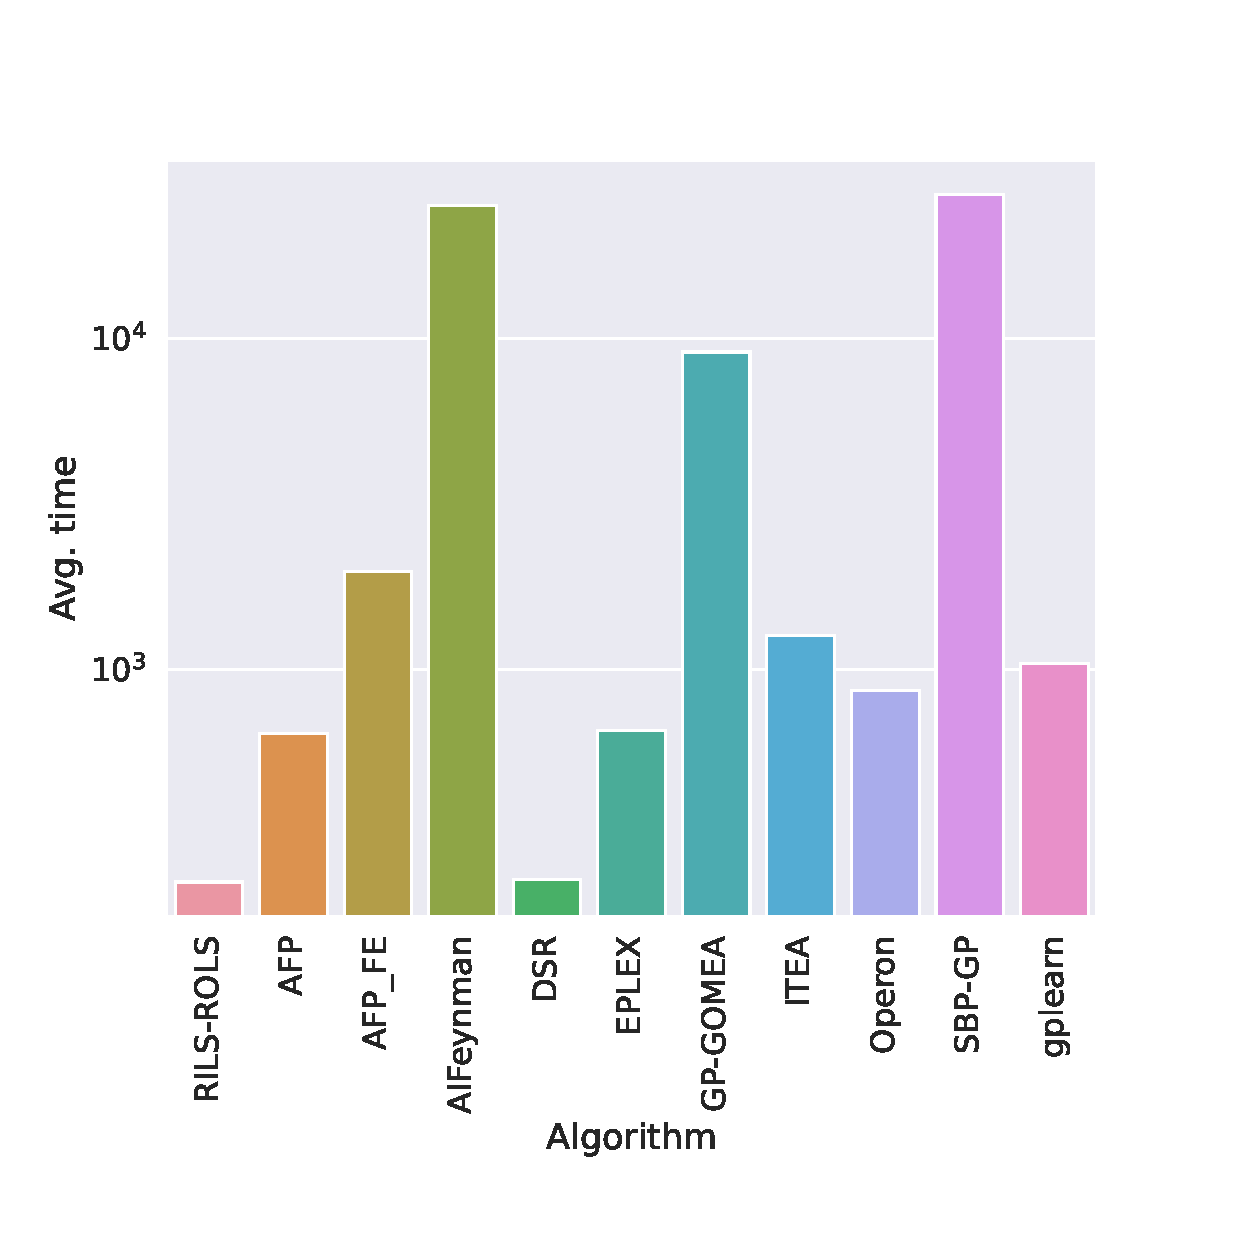
\includegraphics[width=190pt,height=150pt]{plots/time-avg-noise0.0.eps}
		\caption{No noise}
		\label{fig:noNoise-time}
	\end{subfigure}
	\hfill
	\begin{subfigure}[b]{0.47\textwidth}
		
		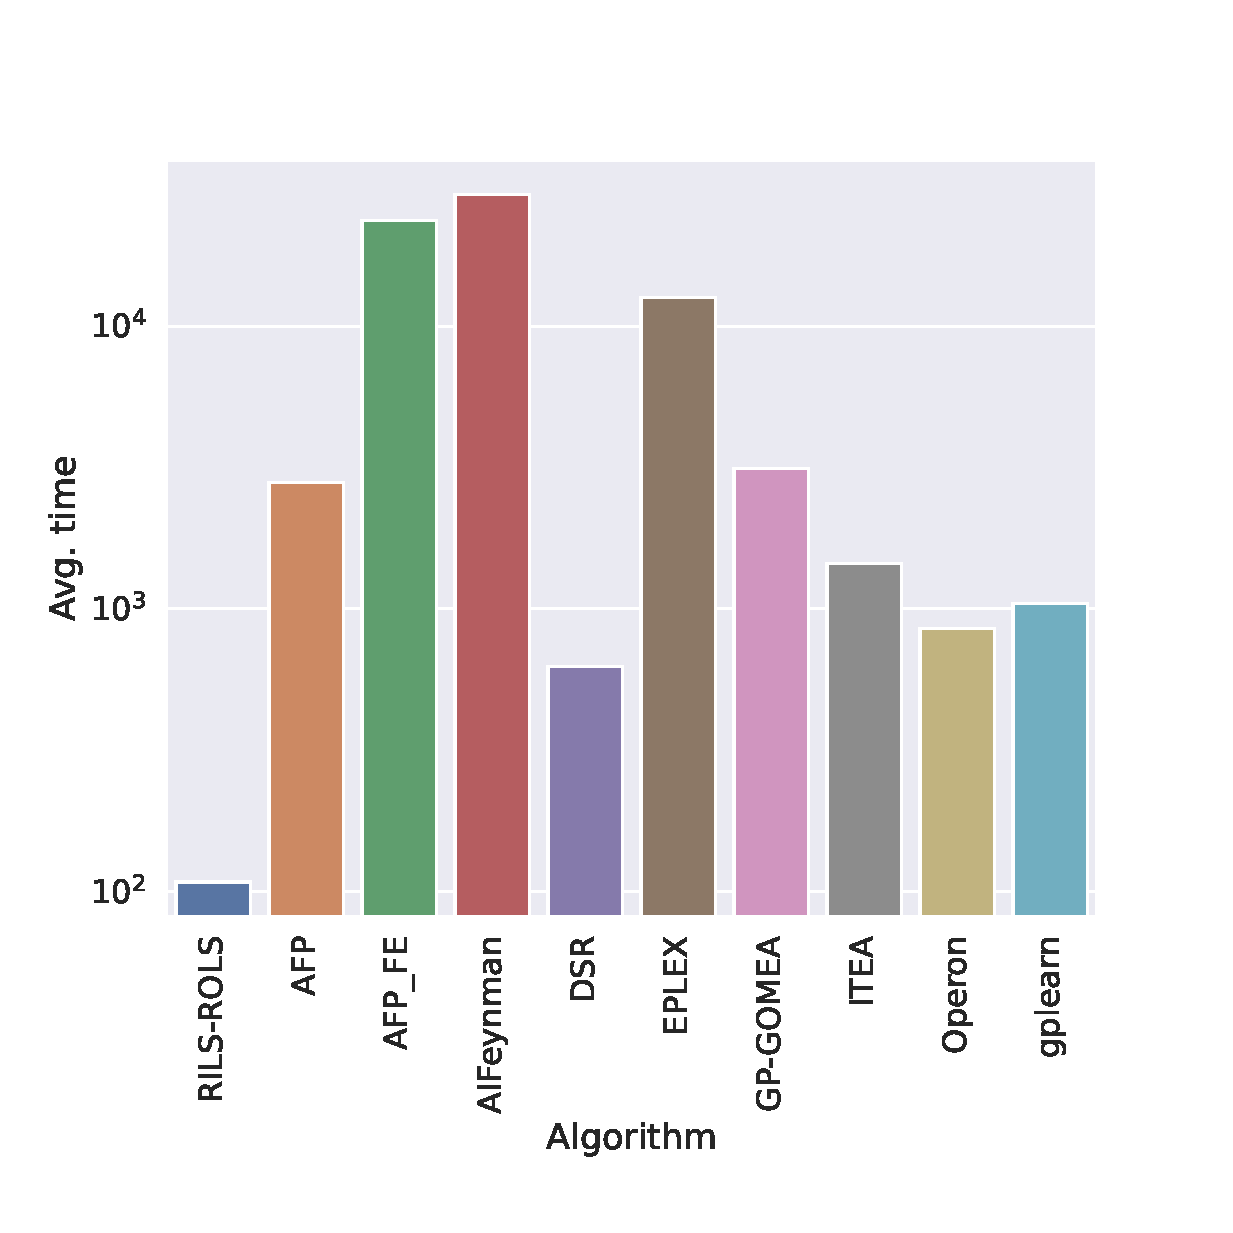
\includegraphics[width=190pt,height=150pt]{plots/time-avg-noise0.001.eps}
		\caption{Level of noise equal to 0.001}
		\label{fig:noise0.001-time}
	\end{subfigure}
	\centering
	\begin{subfigure}[b]{0.47\textwidth}
		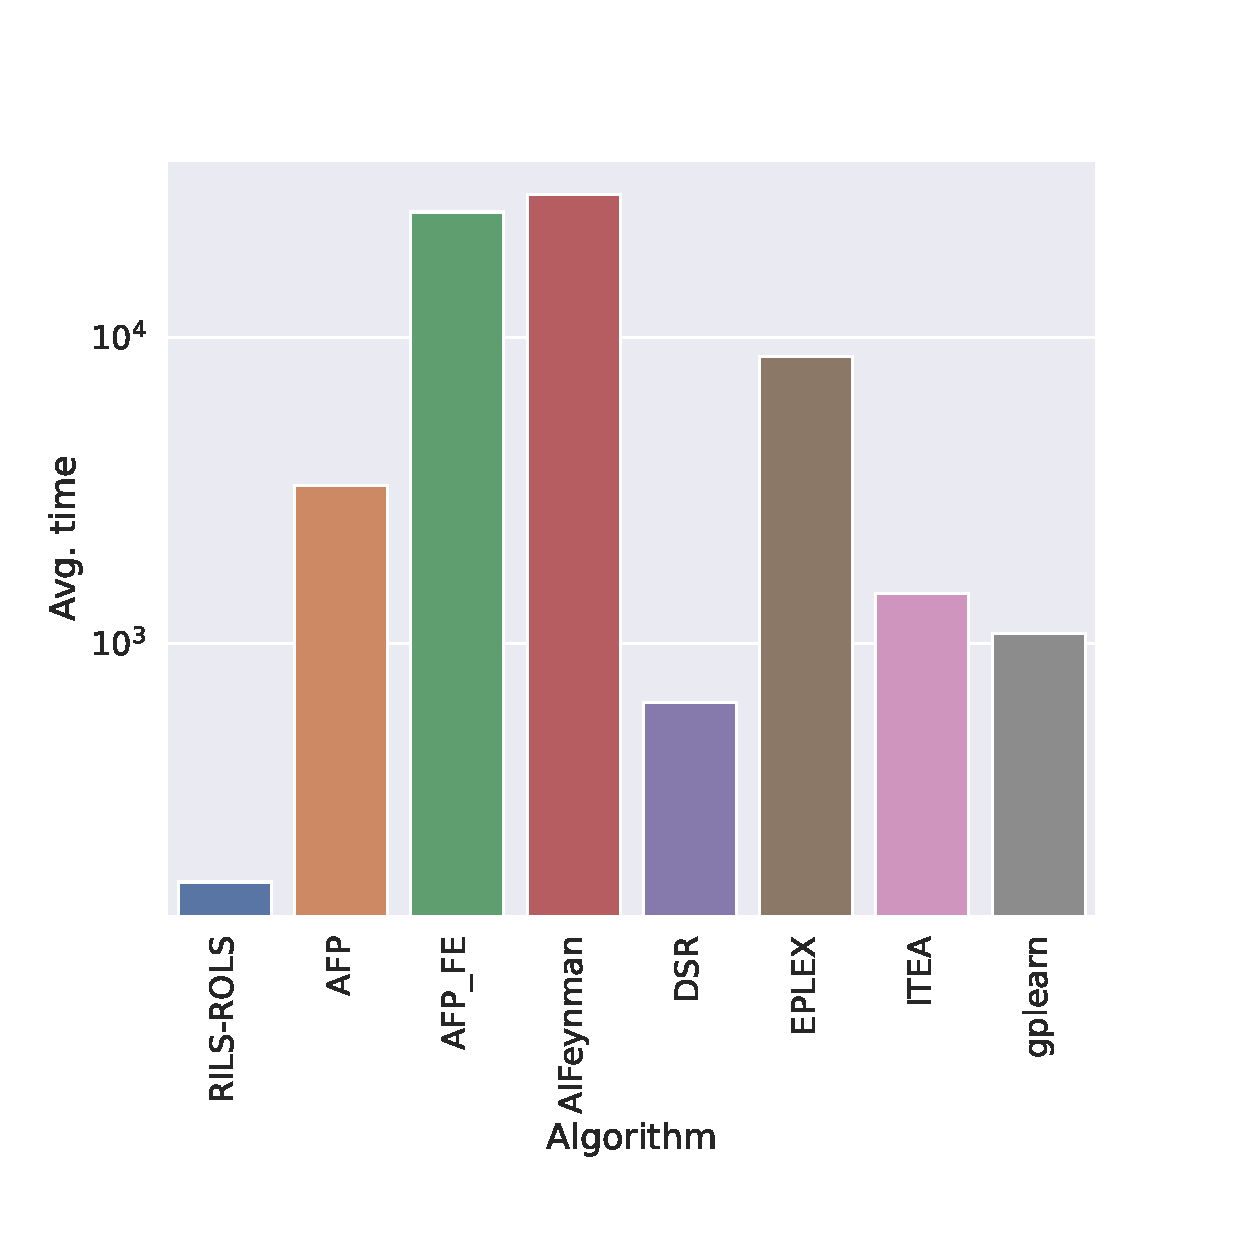
\includegraphics[width=190pt,height=150pt]{plots/time-avg-noise0.01.eps}
		\caption{Level of noise equal to 0.01.}
		\label{fig:noise0.01-time}
	\end{subfigure}
	\caption{Average runtime when exact solution is reached (considering only algorithms whose exact percentage is at least 5\% of all runs).}
	\label{fig:time-avg-exact-noise}
\end{figure}

Figure~\ref{fig:time-avg-exact-noise} compares the methods w.r.t. average runtimes (in seconds) when the exact solution is reached. We do not consider methods whose exact percentage is too low, i.e., below 5\%. Methods are labeled on the $x$-axis, while respective average runtimes are shown on the $y$-axis. (Note that $y$-axis is logarithmically scaled.) The following conclusions are drawn from these results.

\begin{itemize}
	\item When considering instance problems without noise, the lowest average runtime is reported for the \textsc{RILS}-\textsc{ROLS} algorithm (228 seconds). A slightly worse runtime is obtained by the \textsc{DSR} algorithm (232 seconds). Note that the relative exact percentage produced by the \textsc{RILS}-\textsc{ROLS} is far better than \textsc{DSR} (60.62\% versus 19.71\%). All the remaining approaches deliver an order of magnitude larger average runtime than that of \textsc{RILS}-\textsc{ROLS} and \textsc{DSR} methods..   
	\item  When considering instances with the noise level of 0.001, the lowest average runtime to obtain the exact model is again delivered by \textsc{RILS}-\textsc{ROLS} algorithm (108 seconds). The second best runtime is produced by \textsc{DSR}, but this time it is significantly longer (622 seconds) compared to \textsc{RILS-ROLS}. 
	\item When considering instance problems with the noise level of 0.01, the conclusion is similar to the previous one. 
\end{itemize}

\subsection{Statistical evaluation}

In order to check the statistical significance of the results w.r.t.\ competitor approaches, we employed the standard statistical methodology. To do so, we have compared the results of \textsc{RILS}-\textsc{ROLS} to 14 other approaches over all algorithm runs on problem instances from both ground-truth benchmark sets, \textsc{Feynman} and \textsc{Strogatz}. The successful run means that the corresponding algorithm found the exact model. Having 1300 runs involved, this means that the maximal number of successful runs is 1300. 

\emph{Important note. Exact model accuracy of \textsc{RILS-ROLS} is calculated by dividing the number of successful runs with 1300, i.e., the maximal possible number of successful runs. 
On the other hand, the exact model accuracy of methods revised in \texttt{SRBench} was calculated in a different way. First, the accuracy of each of 130 considered instances was calculated by dividing the number of successful runs with the number of runs that finished their execution. This means that, for example, if an instance was run 10 times, giving 4 successful models, but failing to finish 2 runs due to memory exhaustion or an other OS issue, the accuracy would be 50\% (4/8) instead of 40\% (4/10). Further, these individual accuracies were averaged. 
We do not believe this was the right way to calculate the accuracy because this allows one to have a high-accuracy method with a low number of successful runs. For example, if method A finishes all of its runs, out of which 650 are successful, its total accuracy will be 50\%. On the other hand, one can have method B that finishes instance execution in only 4 out of 10 runs, giving 2 successful models each time; its per-instances accuracy will be 50\%, and after averaging across all instances, it will also be 50\%. Methods A and B will therefore have the same overall accuracy, although method A reached 650 correct solutions, while method B reached only 260. Also note that our calculation cannot overestimate \textsc{RILS-ROLS} exact model accuracy, since the denominator is always maximal (1300). In essence, non-finished runs are counted as non-successful.} 

We first conducted the omnibus rank-based Friedman’s test for all approaches. 
The number of ranks is 1300, i.e., a separate rank is calculated for each run of each method. The rank is based on the value of the indicator variable, which takes 1 if the method delivers the correct model in a given run; otherwise it takes value 0, no matter if the method has finished and delivered an incorrect model, or the method did not finish at all. The ranks are further averaged and used to test the null hypothesis, which states that there are statistical differences between the average ranks of all competitors. 
In the case the null hypothesis $H_0$ was rejected, pairwise comparisons were further performed by using the Nemenyi post-hoc test~\cite{pohlert2014pairwise}. The outcome is represented by means of critical difference (CD) plots. 
 
In each CD plot, 15 competitors are placed on the horizontal axis according to their average ranking. Thereafter, the CD score is computed for the significance level of 0.05. If the difference is small enough, meaning that no statistical difference is detected, a horizontal bar that links statistically equal approaches is drawn. This analysis is done for all three levels of noise, and the corresponding CD plots are shown in Figures~\ref{fig:CDplots-no-noise}-\ref{fig:CDplots-noise0.01}.

\begin{figure}[!h]
	\centering
		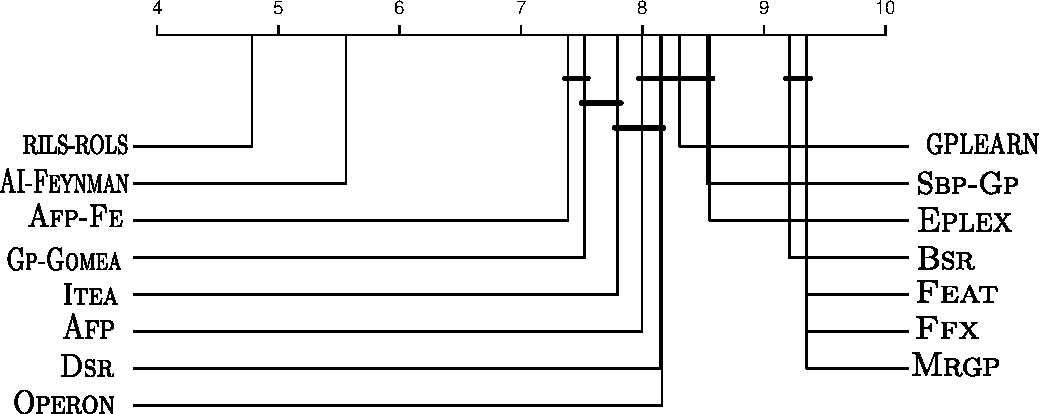
\includegraphics[width=350pt]{plots/Feynman_strogatz_noise_0_0-expanded.pdf}
		\caption{CD plots for no-noise scenario}
		\label{fig:CDplots-no-noise}
\end{figure}
	
\begin{figure}[!h]
	
	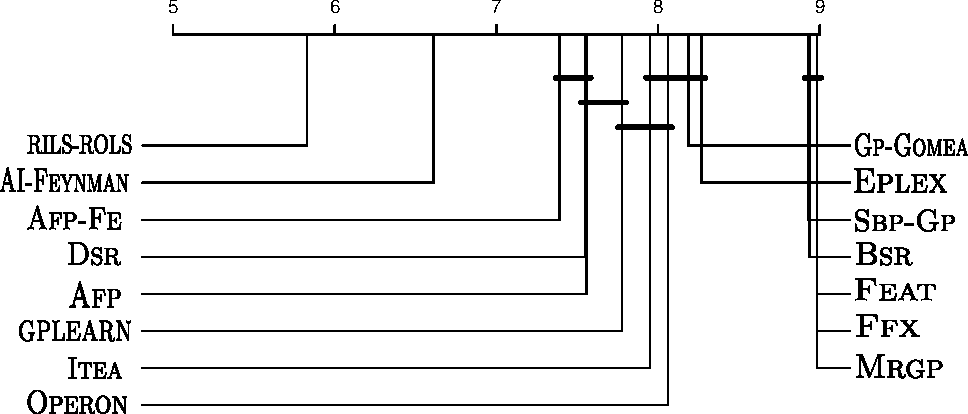
\includegraphics[width=350pt]{plots/Feynman_strogatz_noise_0_001-expanded.pdf}
	\caption{CD plots for noise level 0.001}
	\label{fig:CDplots-noise0.001}
\end{figure}
	
	\begin{figure}[!h]
		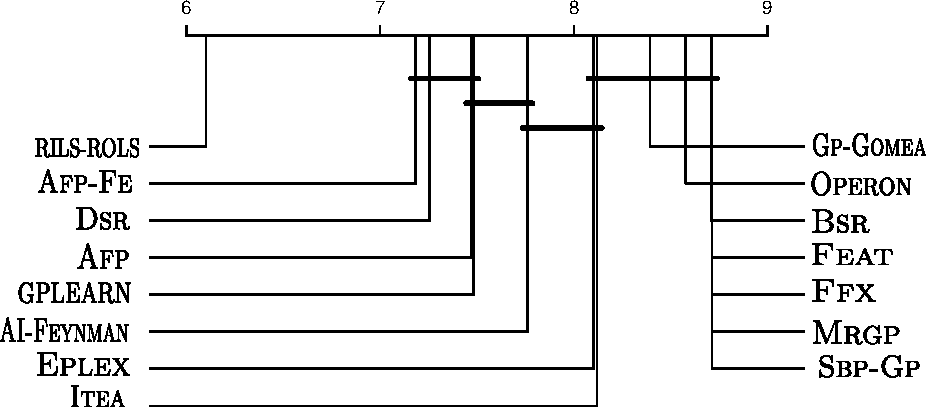
\includegraphics[width=350pt]{plots/Feynman_strogatz_noise_0_01-expanded.pdf}
		\caption{CD plots for noise level 0.01. }
		\label{fig:CDplots-noise0.01}
	\end{figure}

The following conclusions may be drawn.

\begin{itemize}
	\item  Concerning the no-noise scenario, the \textsc{RILS}-\textsc{ROLS} method returns the best average ranking in terms of the number of obtained exact models over all runs.  The second best average ranking is achieved by the \textsc{AI-Feynman} algorithm. There is a statistically significant difference between these two approaches. The third best approach is \textsc{APF-FE},  which is far behind both \textsc{RILS}-\textsc{ROLS} and \textsc{AI-Feynman} w.r.t.\ delivered average ranking.  
	\item  For noise 0.001, the situation is similar. The \textsc{RILS}-\textsc{ROLS} method again obtains the best average ranking. The second best ranking is obtained by the \textsc{AI-Feynman} algorithm. There is a statistically significant difference between the results obtained by these two approaches. The third best approach is \textsc{AFP-FE}, which performs statistically worse than \textsc{AI-Feynman}.  
	\item  When the noise level is 0.01, the \textsc{RILS-ROLS} method is significantly better than other methods. The second best is \textsc{AFP-FE}, followed by \textsc{DSR}, and \textsc{AFTP}. The latter three approaches perform statistically equally. \textsc{AI-Feynman} is fourth, as is \textsc{gplearn}. Note that the average ranking of the \textsc{AI-Feynman} method declines significantly with high noise, which is not the case with the \textsc{RILS}-\textsc{ROLS} method.   
	
\end{itemize}

\subsection{Scalability of \textsc{RILS}-\textsc{ROLS} algorithm}\label{sec:scalability-rils-rols}

In this section we study the scalability of \textsc{RILS-ROLS} w.r.t. size of instance problems under different levels of noise.
Since we do not compare \textsc{RILS-ROLS} to other competitors here, but just assess method scalability and sensitivity to noise, experimental setup is different. First, we run each instance only once -- note that there are 5 randomly generated instances for each of 47 combinations (size, variable count). Second, the exit criteria are different: 1) maximal running time is 300 seconds instead of 1 hour, and 2) maximal number of fitness evaluations is 100,000 instead of 1,000,000. 
As before, the test set takes 25\% of total data. 
For the sake of having a simpler presentation, we split the instances from the \textsc{Random} benchmark into three parts as follows: 
\begin{itemize}
	\item \textit{Small-sized instances}: instances with solution size from 3 to 7.
	\item \textit{Medium-sized instances}: those with size from 8 to 11.
	\item \textit{Large-sized instances}: instances with size from 12 to 15. 
\end{itemize}

The results are displayed in Figure~\ref{fig:compExact_noise_size}, grouped in accordance to the above-mentioned parts ($x$-axis). The exact solution accuracy of \textsc{RILS}--\textsc{ROLS} is shown on the $y$-axis.   

\begin{center}
	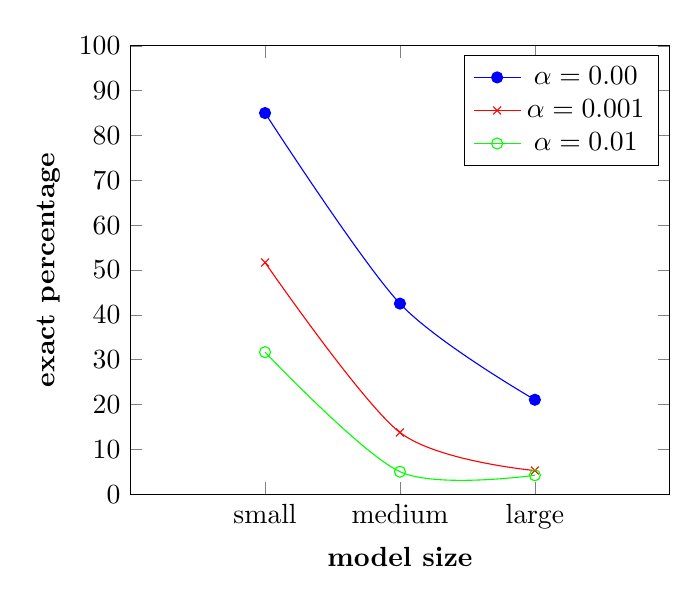
\begin{tikzpicture}
		\begin{axis}[
			xlabel=\textbf{model size},
			ylabel=\textbf{exact percentage},
			xmin=0, xmax=4,
			ymin=0, ymax=100,
			xtick={1,2,3},
			xticklabels={small,medium,large},   % <---
			ytick={0,10,...,100}
			]
			\addplot[smooth,mark=*,blue] plot coordinates {
				(1,85)
				(2,42.5)
				(3,21.05)
			};
			\addlegendentry{$\alpha=0.00$}
			
			\addplot[smooth,color=red,mark=x]
			plot coordinates {
				(1,51.67)
				(2,13.75)
				(3,5.26)
			};
			\addlegendentry{$\alpha=0.001$}
			
			\addplot[smooth,color=green,mark=o]
			plot coordinates {
				(1,31.67)
				(2,5)
				(3,4.21)
			};
			\addlegendentry{$\alpha=0.01$}
		\end{axis}
	\end{tikzpicture}
	\captionof{figure}{Exact solution percentages for varying levels of noise and formulae sizes}
	\label{fig:compExact_noise_size}
\end{center}

This leads to the following conclusions:  

\begin{itemize}
	\item  As expected, the accuracy (exact percentage) is highest for small-sized instances -- it is sightly below 90\% in a no-noise scenario. For noisy data, the accuracy naturally decreases as the level of noise increases. For example, on the small-sized problem instances with the noise level of 0.001 and 0.01, the accuracy achieved by \textsc{RILS}-\textsc{ROLS} is still reasonably high, at about 55\%~ and 34\%, respectively. 
	\item For medium-sized instances when there is no noise, the exact percentage rate is slightly below 50\%. It also decreases as the level of noise increases -- for the highest level of noise (0.01), the accuracy of the \textsc{RILS}-\textsc{ROLS} method is just about 6\%. 
	\item For large-sized instance problems where no noise is included, the exact percentage is about 25\%, which means that the increase in size affects the algorithm's performance, but not dramatically.  
	
	\item We can conclude that increased formula size and noise level jointly contribute to deterioration of overall \textsc{RILS-ROLS} accuracy, which is expected and natural. The diagram suggests that this deterioration behaves similarly across different levels of noise when instance size changes from small to medium almost linearly, and with almost exact slope. On the other hand, the relative deterioration of accuracy under no-noise level, when going from a medium to a large instance, is higher than under noisy data. A possible explanation for this is that the exact solution accuracy of medium instances has already significantly deteriorated in a noisy scenario. A further increase in size therefore does not have a significant impact. 
\end{itemize}
	
Results for $R^2 > 0.999$ accuracy are presented in Figure~\ref{fig:compR2_noise_size}. 

\begin{center}
	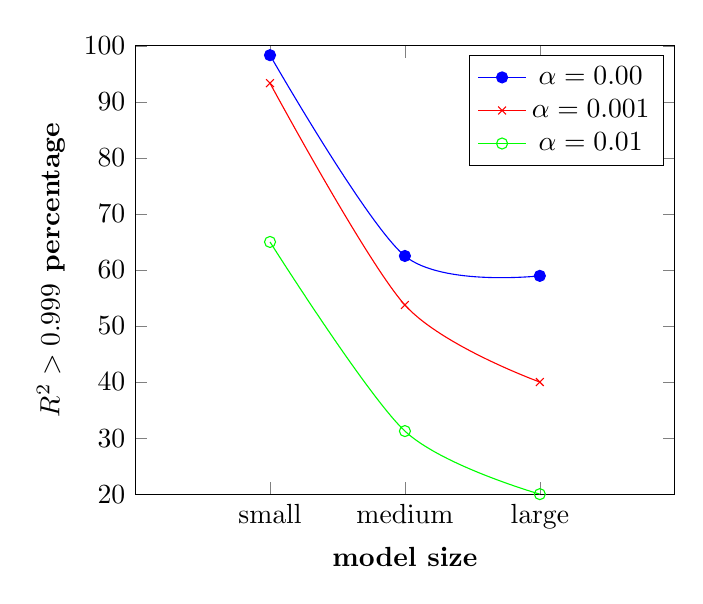
\begin{tikzpicture}
		\begin{axis}[
			xlabel=\textbf{model size},
			ylabel=\textbf{$R^2 > 0.999$ percentage},
			xmin=0, xmax=4,
			ymin=20, ymax=100,
			xtick={1,2,3},
			xticklabels={small,medium,large},   % <---
			ytick={20,30,...,100}
			]
			\addplot[smooth,mark=*,blue] plot coordinates {
				(1,98.33)
				(2,62.5)
				(3,58.95)
			};
			\addlegendentry{$\alpha=0.00$}
			
			\addplot[smooth,color=red,mark=x]
			plot coordinates {
				(1,93.33)
				(2,53.75)
				(3,40)
			};
			\addlegendentry{$\alpha=0.001$}
			
			\addplot[smooth,color=green,mark=o]
			plot coordinates {
				(1,65)
				(2,31.25)
				(3,20)
			};
			\addlegendentry{$\alpha= 0.01$}
		\end{axis}
	\end{tikzpicture}
	\captionof{figure}{Percentages of solutions having $R^2 > 0.999$ for varying levels of noise and formulae sizes}
	\label{fig:compR2_noise_size}
\end{center}

The following conclusions may be drawn from these results:

\begin{itemize}
	
	\item For small-sized instances where no noise is included, \textsc{RILS}-\textsc{ROLS} delivers almost the perfect score. In the presence of low noise (0.001), this percentage is still holding high, at about 95\%. In case when there is a lot of noise (0.01), these percentages deteriorate significantly, but still come at respectable 66\%. 
	
	\item Concerning medium-sized instances in a no-noise scenario, accuracy is around 65\%. Having low noise does not affect the results considerably. However, under high noise, the impact is significant and very similar to the effect observable in small-sized instances -- it reduces accuracy to just $\approx$30\%.
	
	\item In the case of large-sized instances without noise,  accuracy is around 60\%, which is very small relative deterioration in comparison to middle-sized instances. Not surprisingly, large instances under high noise are the most difficult to solve -- only 20\% reached $R^2 > 0.999$. 
	
\end{itemize}

In the rest of the section, we investigate the sensitivity of \textsc{RILS}-\textsc{ROLS} to the variable count under varying levels of noise. There are three bar plots generated per each level of noise presented in Figures~\ref{fig:compExact_noise_varcnt}. The instances are grouped according to a different variable count ($x$-axis). Exact percentages for each group are shown on the $y$-axis.

\begin{figure}[!h]
	
	\begin{subfigure}[b]{0.45\textwidth}
		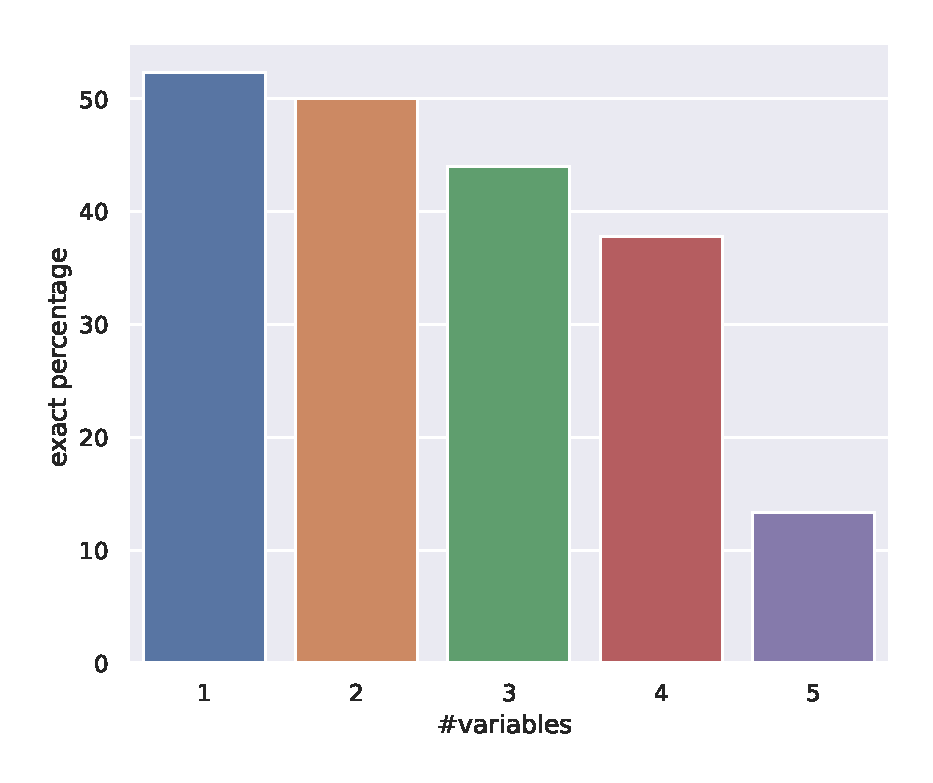
\includegraphics[width=180pt,height=140pt]{plots/numvars_vs_exact_correct_no_noise.eps}
		\caption{No noise}
		\label{fig:noNoise}
	\end{subfigure}
	\hfill
	\begin{subfigure}[b]{0.45\textwidth}
		
		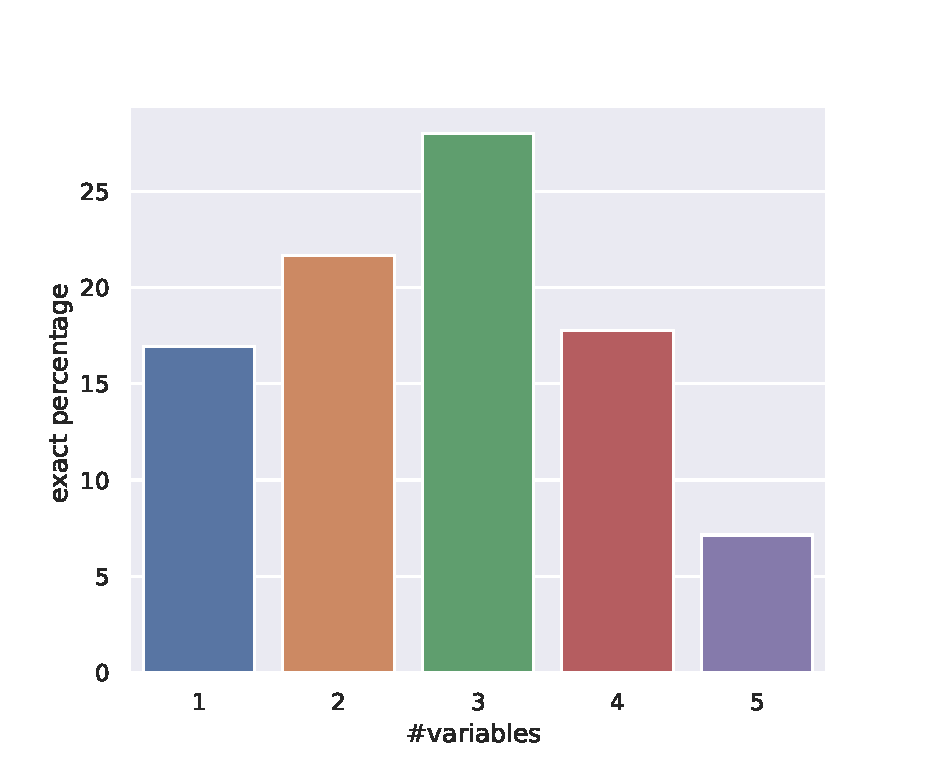
\includegraphics[width=180pt,height=140pt]{plots/numvars_vs_exact_correct_noise0_001.eps}
		\caption{Level of noise equal to 0.001}
		\label{fig:noise0.001}
	\end{subfigure}
	\centering
	\begin{subfigure}[b]{0.40\textwidth}
		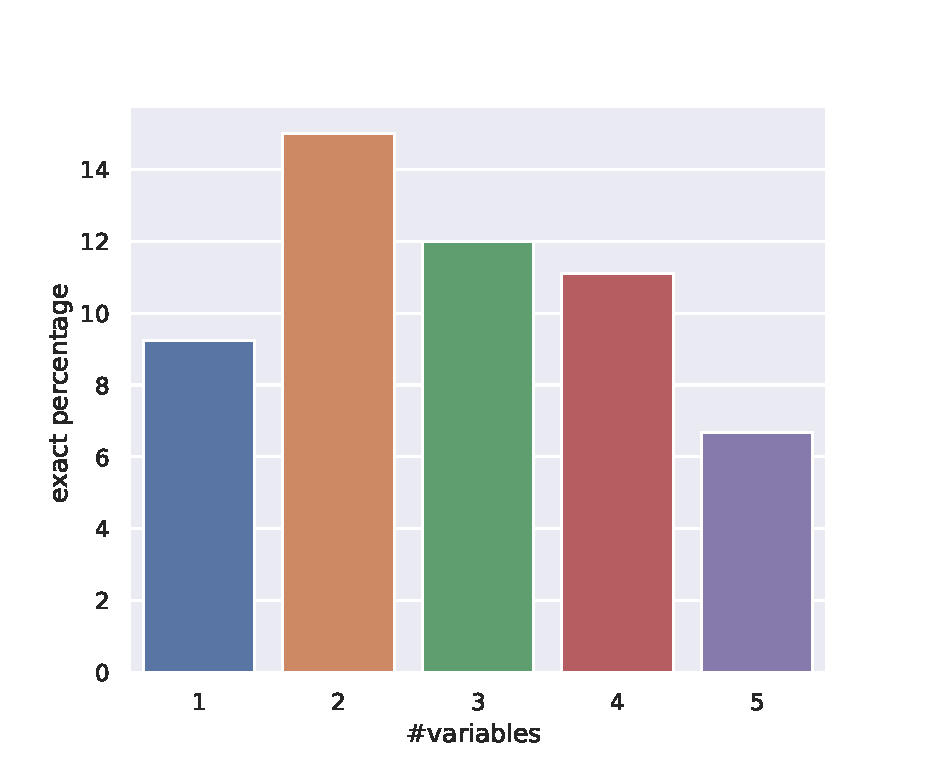
\includegraphics[width=180pt,height=140pt]{plots/numvars_vs_exact_correct_noise0_01.eps}
		\caption{Level of noise equal to 0.01.}
		\label{fig:noise0.01}
	\end{subfigure}
	\caption{Exact solution percentages for varying levels of noise and variable counts.}
	\label{fig:compExact_noise_varcnt}
\end{figure}

These results lead to the following conclusions:

\begin{itemize}
	\item For data without noise, the exact percentage of \textsc{RILS}-\textsc{ROLS} slightly decreases as the  number of variables increases. 
	\item The exact percentage drops off in the presence of a higher level of noise. As expected, higher noise means smaller exact percentage.
	\item Interestingly, in the presence of noise in data, the highest exact percentages are not obtained for instances with a single input variable, but for those with two or three. This is probably due to the expected level of \emph{non-linearity} in instances. Namely, when the size of an instance is fixed, instances with fewer input variables will have to use more operations to compensate for the lack of input variables. Note that expression size is calculated simply by counting all nodes in the expression tree, whether these nodes are operations, constants or variables. Therefore, instances with fewer variables will use operations and their compositions more heavily, paving the way to a more \emph{difficult} functional structure. 
	The reason this is not an issue for no-noisy data is because \textsc{RILS-ROLS} will have to \emph{wander} less -- there will not be so many contradictory search directions as with noisy data.
\end{itemize}

\textsc{RILS}-\textsc{ROLS} running times for \textsc{Random} benchmark are shown in Figure~\ref{fig:runtime_rils_rols}. Instances are grouped w.r.t.\ the number of variables ($x$-axis). 
As one could expect, the average running time increases with the increase in the number of variables. 
\textsc{RILS-ROLS} usually terminates because the maximal number of fitness evaluation is reached (100,000) with average running times below 300 seconds, which is the time-based exit criterion.

\begin{figure}[!h]
	\begin{subfigure}[b]{0.45\textwidth}
		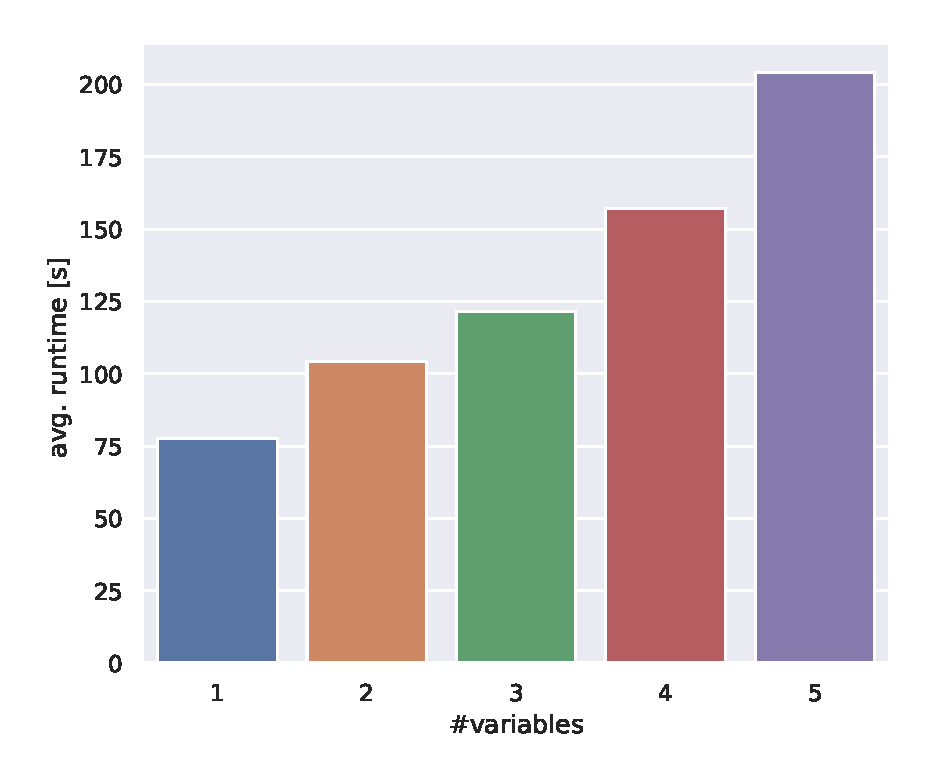
\includegraphics[width=180pt,height=140pt]{plots/numsize_vs_time_no_noise.eps}
		\caption{No noise}
		\label{fig:time-no-noise}
	\end{subfigure}
	\hfill
	\begin{subfigure}[b]{0.45\textwidth}
		
		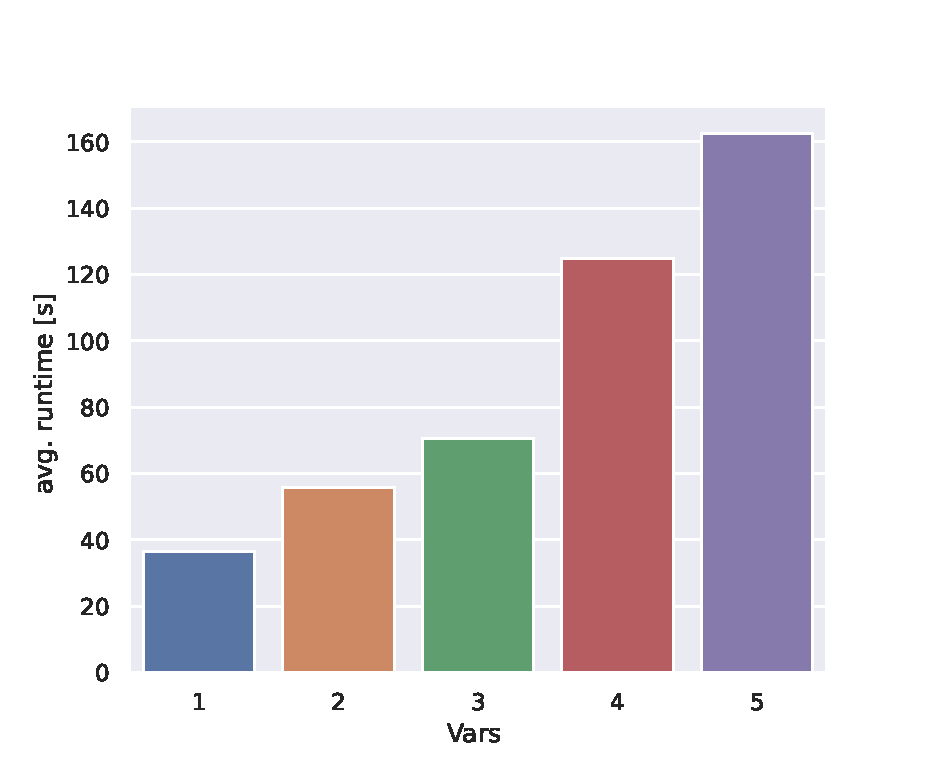
\includegraphics[width=180pt,height=140pt]{plots/vars_vs_time_noise0_001.eps}
		\caption{Level of noise equal to 0.001}
		\label{fig:time-noise0.001}
	\end{subfigure}
	\centering
	\begin{subfigure}[b]{0.40\textwidth}
		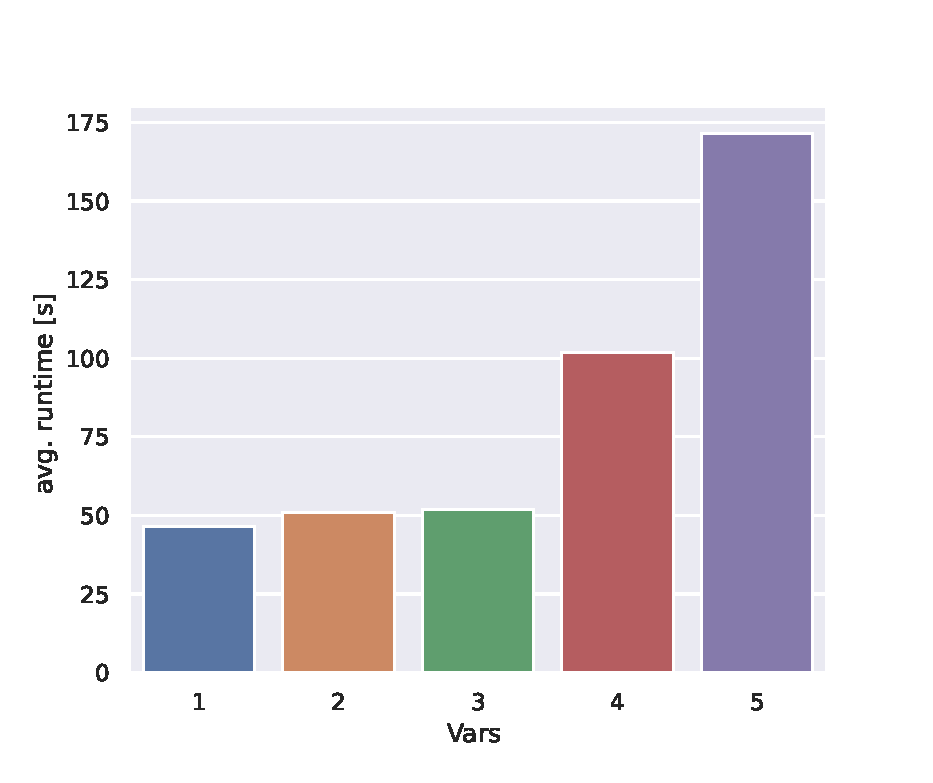
\includegraphics[width=180pt,height=140pt]{plots/vars_vs_time_noise0_01.eps}
		\caption{Level of noise equal to 0.01.}
		\label{fig:time-noise0.01}
	\end{subfigure}
	\caption{Average runtime comparisons for varying levels of noise and variable counts.}
	\label{fig:runtime_rils_rols}
\end{figure}


\section{Conclusions and future work}\label{sec:conclusions}

In this paper we dealt with solving the well-known symbolic regression (SR)  problem.  
We proposed a meta-heuristic approach called \textsc{RILS}-\textsc{ROLS}, built upon the iterated local search (ILS) scheme. The crucial element of this scheme is the ordinary least square method (OLS), used to efficiently determine the best-fitting linear coefficients within solution equations. 
Another key aspect is the utilization of a carefully constructed fitness function which combines three important measures of the solution: RMSE, $R^2$, and solution size. 
Further, we designed an efficient local search that systematically explores the solution space around the candidate solution.

The \textsc{RILS-ROLS} method is compared to 14 other competing methods from the literature on two ground-truth benchmark sets from the literature: \textsc{Feynman} and \textsc{Strogatz}. Experimental evaluation confirmed the quality of our method -- \textsc{RILS-ROLS} produced the best average ranking results in terms of exact model accuracy under varying levels of noise in data. 
Our algorithm was able to find the right model with 60.62\%, 42.08\%, and 34.77\% accuracy under no-noise, low-level noise and high-level noise, respectively. The second best approach, \textsc{AI-Feynman}, obtains fairly worse percentages: 52.65\%, 31.89\%, and 20\%. 

In addition to well-known benchmarks from the literature, we introduced a new non-biased benchmark set of randomly generated instances.  %, labeled by \textsc{Random}. 
This benchmark was used to test \textsc{RILS}-\textsc{ROLS} scalability, by varying the size of the model and the number of variables. 

In the future, one could think of constructing a hybrid of \textsc{RILS-ROLS} method with some other meta-heuristics to further boost the quality of the obtained results. For example, replacing the ILS scheme of \textsc{RILS-RILS} with a more general Variable neighborhood search (VNS) scheme is a reasonable option. Also, \textsc{RILS-ROLS} could be used to solve practical problems from various domains. For example, it can be used in physics or chemistry to help set up reasonable hypotheses or obtain valuable insights into obtained experimental evaluations. Another improvement direction is incorporating top-level constraints into the method. For example, if one knows that the modeled function needs to be monotonically decreasing or differentiable, or both, this knowledge can be used to alter the search -- eliminate inadequate parts of the search space (hard constraint) or more subtly penalize this behavior through fitness function (soft constraint). 

\section*{Appendix - \textsc{RILS}-\textsc{ROLS} Python package}\label{sec:appendix-1}

\textsc{RILS-ROLS} algorithm is available for installation in the well-known Python package repository \url{https://pypi.org}, so it can be easily installed by typing commands:
\begin{python} 
	pip install rils-rols
\end{python}
\textsc{RILS-ROLS} PyPI project page is available at \url{https://pypi.org/project/rils-rols}. Here, one can find a minimal working example on how to use \textsc{RILS-ROLS}:

\begin{python}
	from rils_rols.rils_rols import RILSROLSRegressor
	from math import sin, log
	
	regr = RILSROLSRegressor()
	
	# toy dataset 
	X = [[3, 4], [1, 2], [-10, 20], [10, 10], [100, 100], [22, 23]]
	y = [sin(x1)+2.3*log(x2) for x1, x2 in X]
	
	# RILSROLSRegressor inherits BaseEstimator (sklearn)
	regr.fit(X, y)
	
	# this prints out the learned model
	print("Final model is "+str(regr.model))
	
	# applies the model to a list of input vectors
	X_test = [[4, 4], [3, 3]]
	y_test = regr.predict(X_test)
	print(y_test) 
\end{python}

Python sources, experimental results and all other \textsc{RILS-ROLS} resources can be found at the project GitHub page \url{https://github.com/kartelj/rils-rols}. 
 

%%%%%%%%%%%%%%%%%%%%%%%%%%%%%%%%%%%%%%%%%%%%%%
%%                                          %%
%% Backmatter begins here                   %%
%%                                          %%
%%%%%%%%%%%%%%%%%%%%%%%%%%%%%%%%%%%%%%%%%%%%%%

\begin{backmatter}

 \section*{Acknowledgments}%% if any
Not applicable.

 \section*{Funding}%% if any
Not applicable.

%\section*{Abbreviations}%% if any
%Text for this section\ldots

  \section*{Availability of data and materials}%% if any
 All accompanying resources regarding this paper can be found in the GitHub repository \url{https://github.com/kartelj/rils-rols}. 

\section*{Ethics approval and consent to participate}%% if any
Not applicable. 

\section*{Competing interests}
The authors declare  no competing interests.

\section*{Consent for publication}%% if any
Not applicable. 

\section*{Authors' contributions}
Both A.K. and M.Dj. contributed to the conception of the work. A.K. worked on the implementation of method and the design of experiments. M.Dj. worked on analysis and discussion of the results, introduction and literature review. 

%\section*{Authors' information}%% if any
%Text for this section\ldots

%%%%%%%%%%%%%%%%%%%%%%%%%%%%%%%%%%%%%%%%%%%%%%%%%%%%%%%%%%%%%
%%                  The Bibliography                       %%
%%                                                         %%
%%  Bmc_mathpys.bst  will be used to                       %%
%%  create a .BBL file for submission.                     %%
%%  After submission of the .TEX file,                     %%
%%  you will be prompted to submit your .BBL file.         %%
%%                                                         %%
%%                                                         %%
%%  Note that the displayed Bibliography will not          %%
%%  necessarily be rendered by Latex exactly as specified  %%
%%  in the online Instructions for Authors.                %%
%%                                                         %%
%%%%%%%%%%%%%%%%%%%%%%%%%%%%%%%%%%%%%%%%%%%%%%%%%%%%%%%%%%%%%

% if your bibliography is in bibtex format, use those commands:
\bibliographystyle{bmc-mathphys} % Style BST file (bmc-mathphys, vancouver, spbasic).
\bibliography{bib}      % Bibliography file (usually '*.bib' )
 
 

%%%%%%%%%%%%%%%%%%%%%%%%%%%%%%%%%%%
%%                               %%
%% Figures                       %%
%%                               %%
%% NB: this is for captions and  %%
%% Titles. All graphics must be  %%
%% submitted separately and NOT  %%
%% included in the Tex document  %%
%%                               %%
%%%%%%%%%%%%%%%%%%%%%%%%%%%%%%%%%%%

%%
%% Do not use \listoffigures as most will included as separate files
 

 
 

%\section*{Additional Files}
%  \subsection*{Additional file 1 --- Sample additional file title}
 %   Additional file descriptions text (including details of how to
 %   view the file, if it is in a non-standard format or the file extension).  This might
 %   refer to a multi-page table or a figure...
 

\end{backmatter}
\end{document}
